\chapter{Anhang}
\label{chap:Anhang}

\begin{figure}[h!]
	\centering
	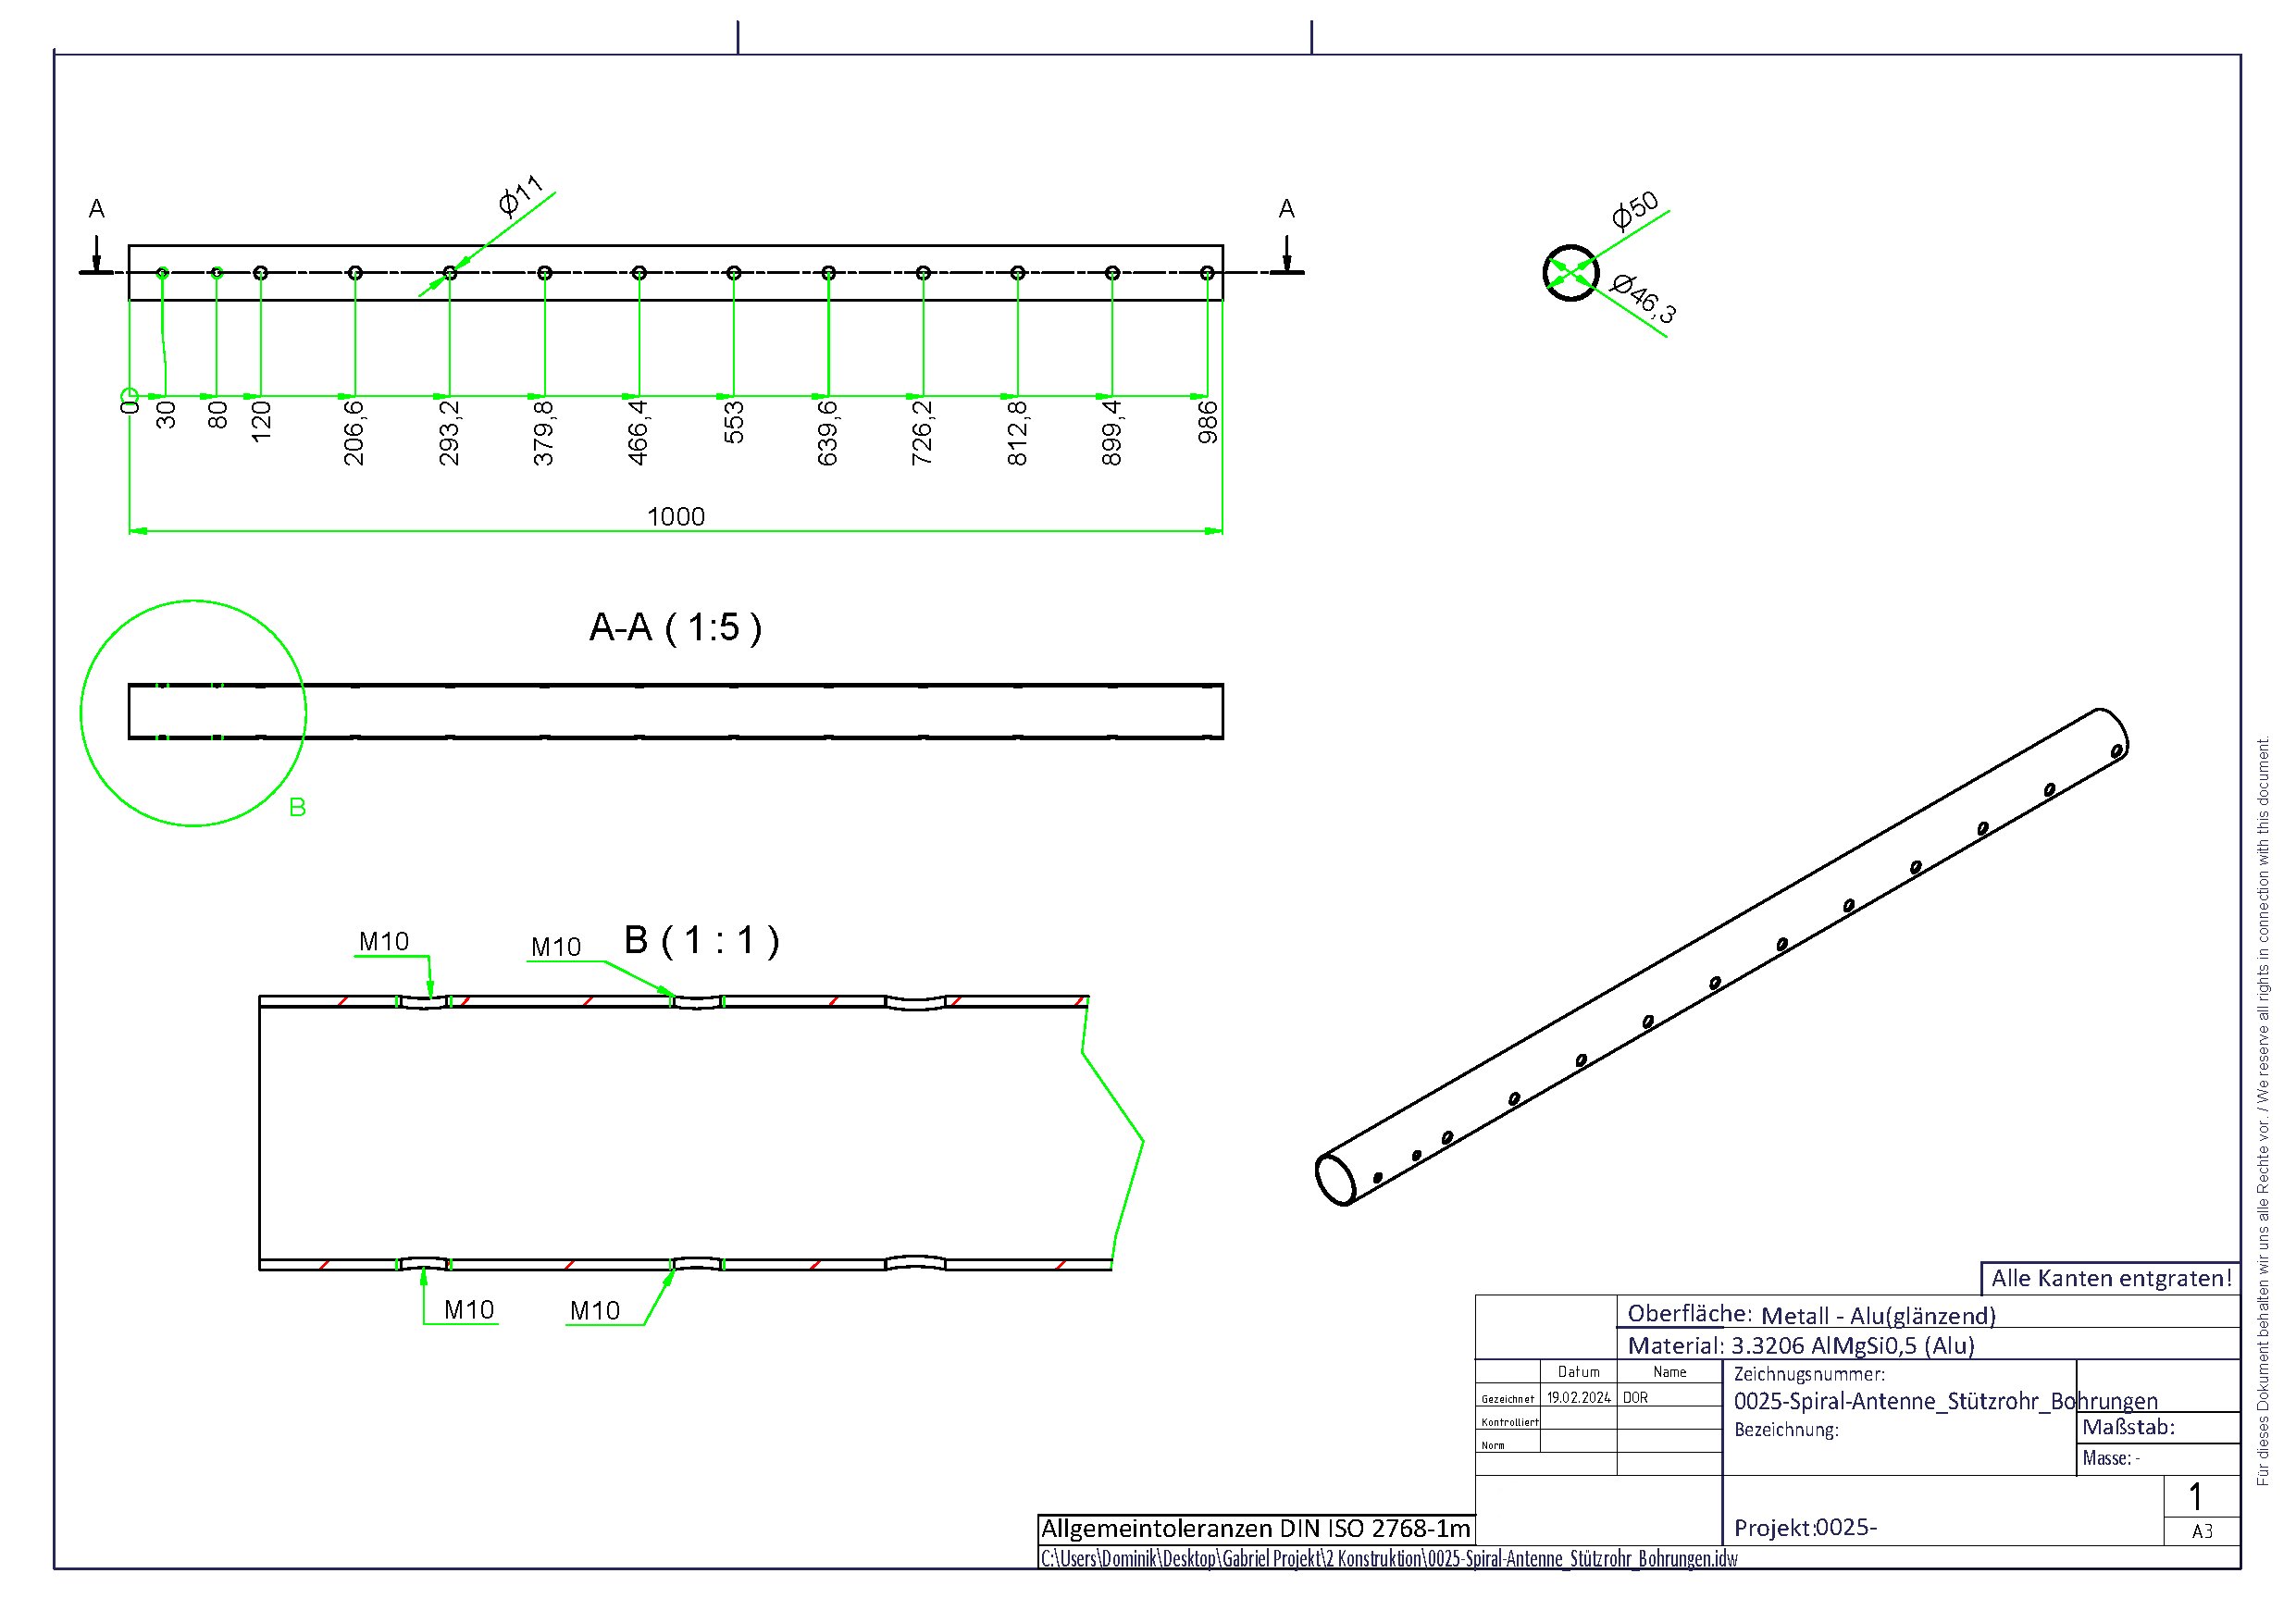
\includegraphics[angle=90,width=\textwidth]{../ref/0025-Spiral-Antenne_St_tzrohr_Bohrungen.pdf}
	\caption{Der Bohrplan des PVC-Rohres}
	\label{fig:PVCU-Rohr-Bohrplan}
\end{figure}

\begin{figure}[h!]
	\centering
	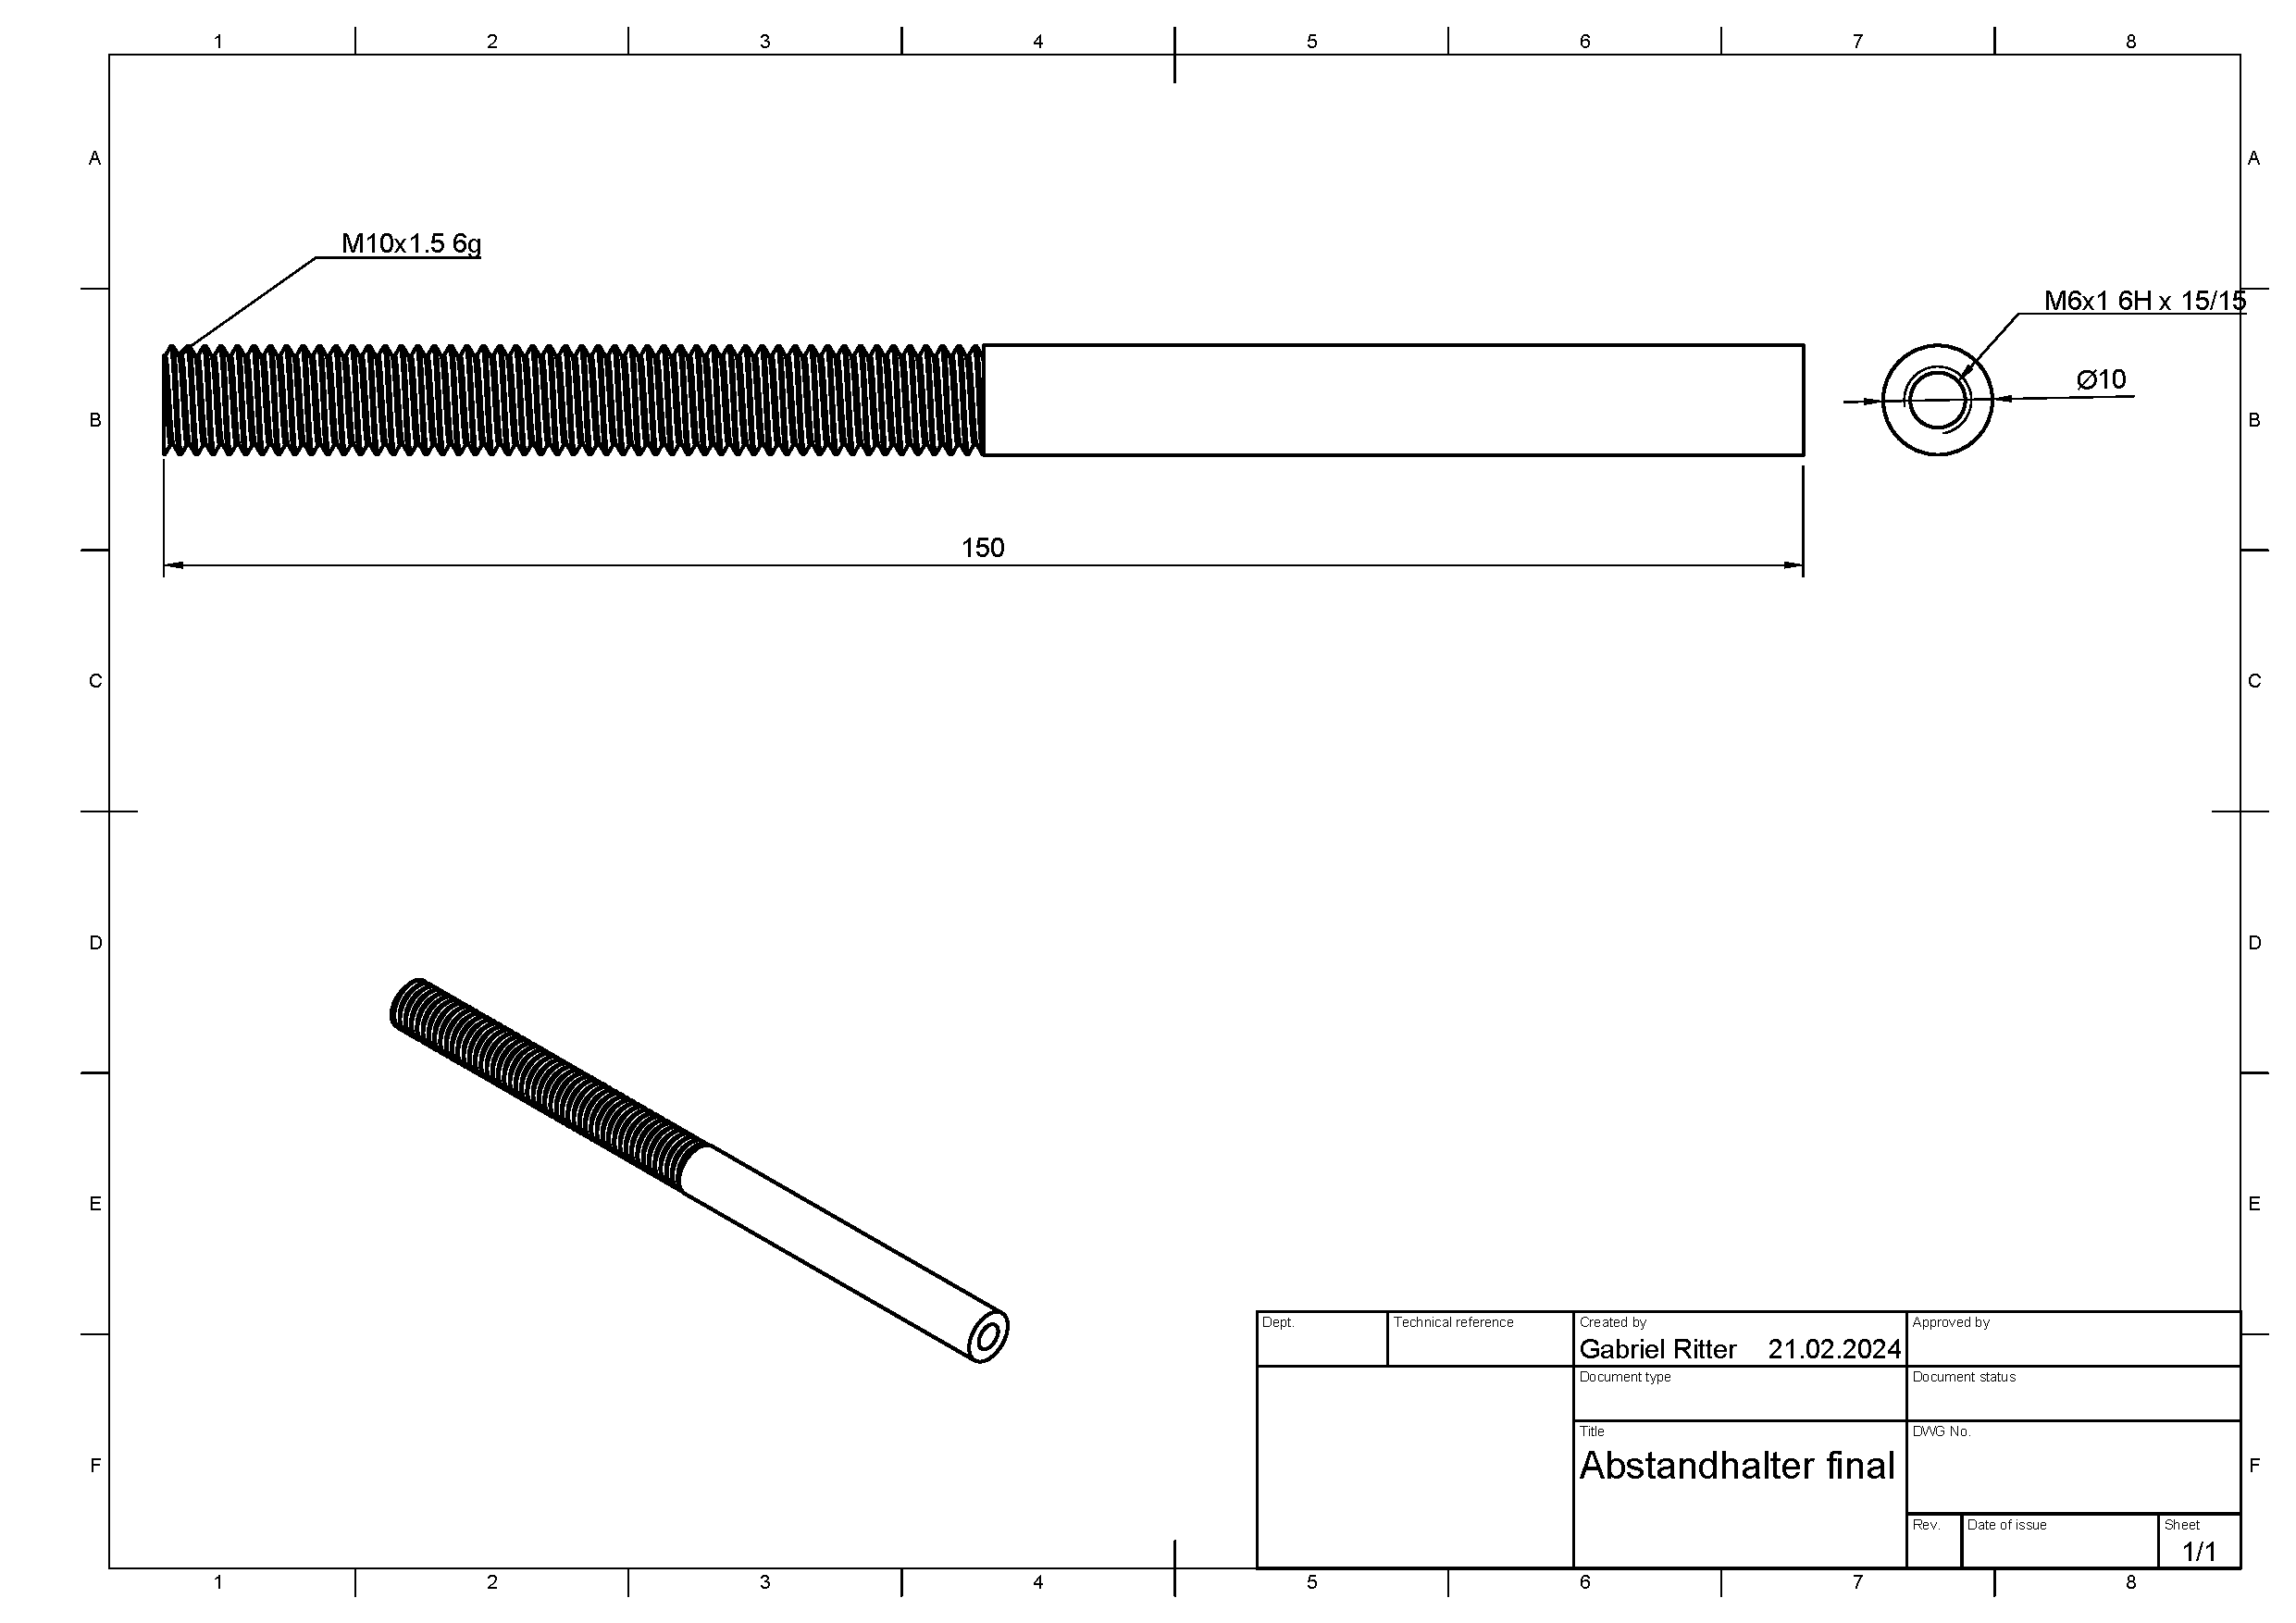
\includegraphics[angle=90,width=\textwidth]{../ref/Abstandhalter final Zeichnung v2.pdf}
	\caption{Zeichnung des Abstandhalters}
	\label{fig:Abstandhalter-Zeichnung}
\end{figure}

\begin{figure}[h!]
	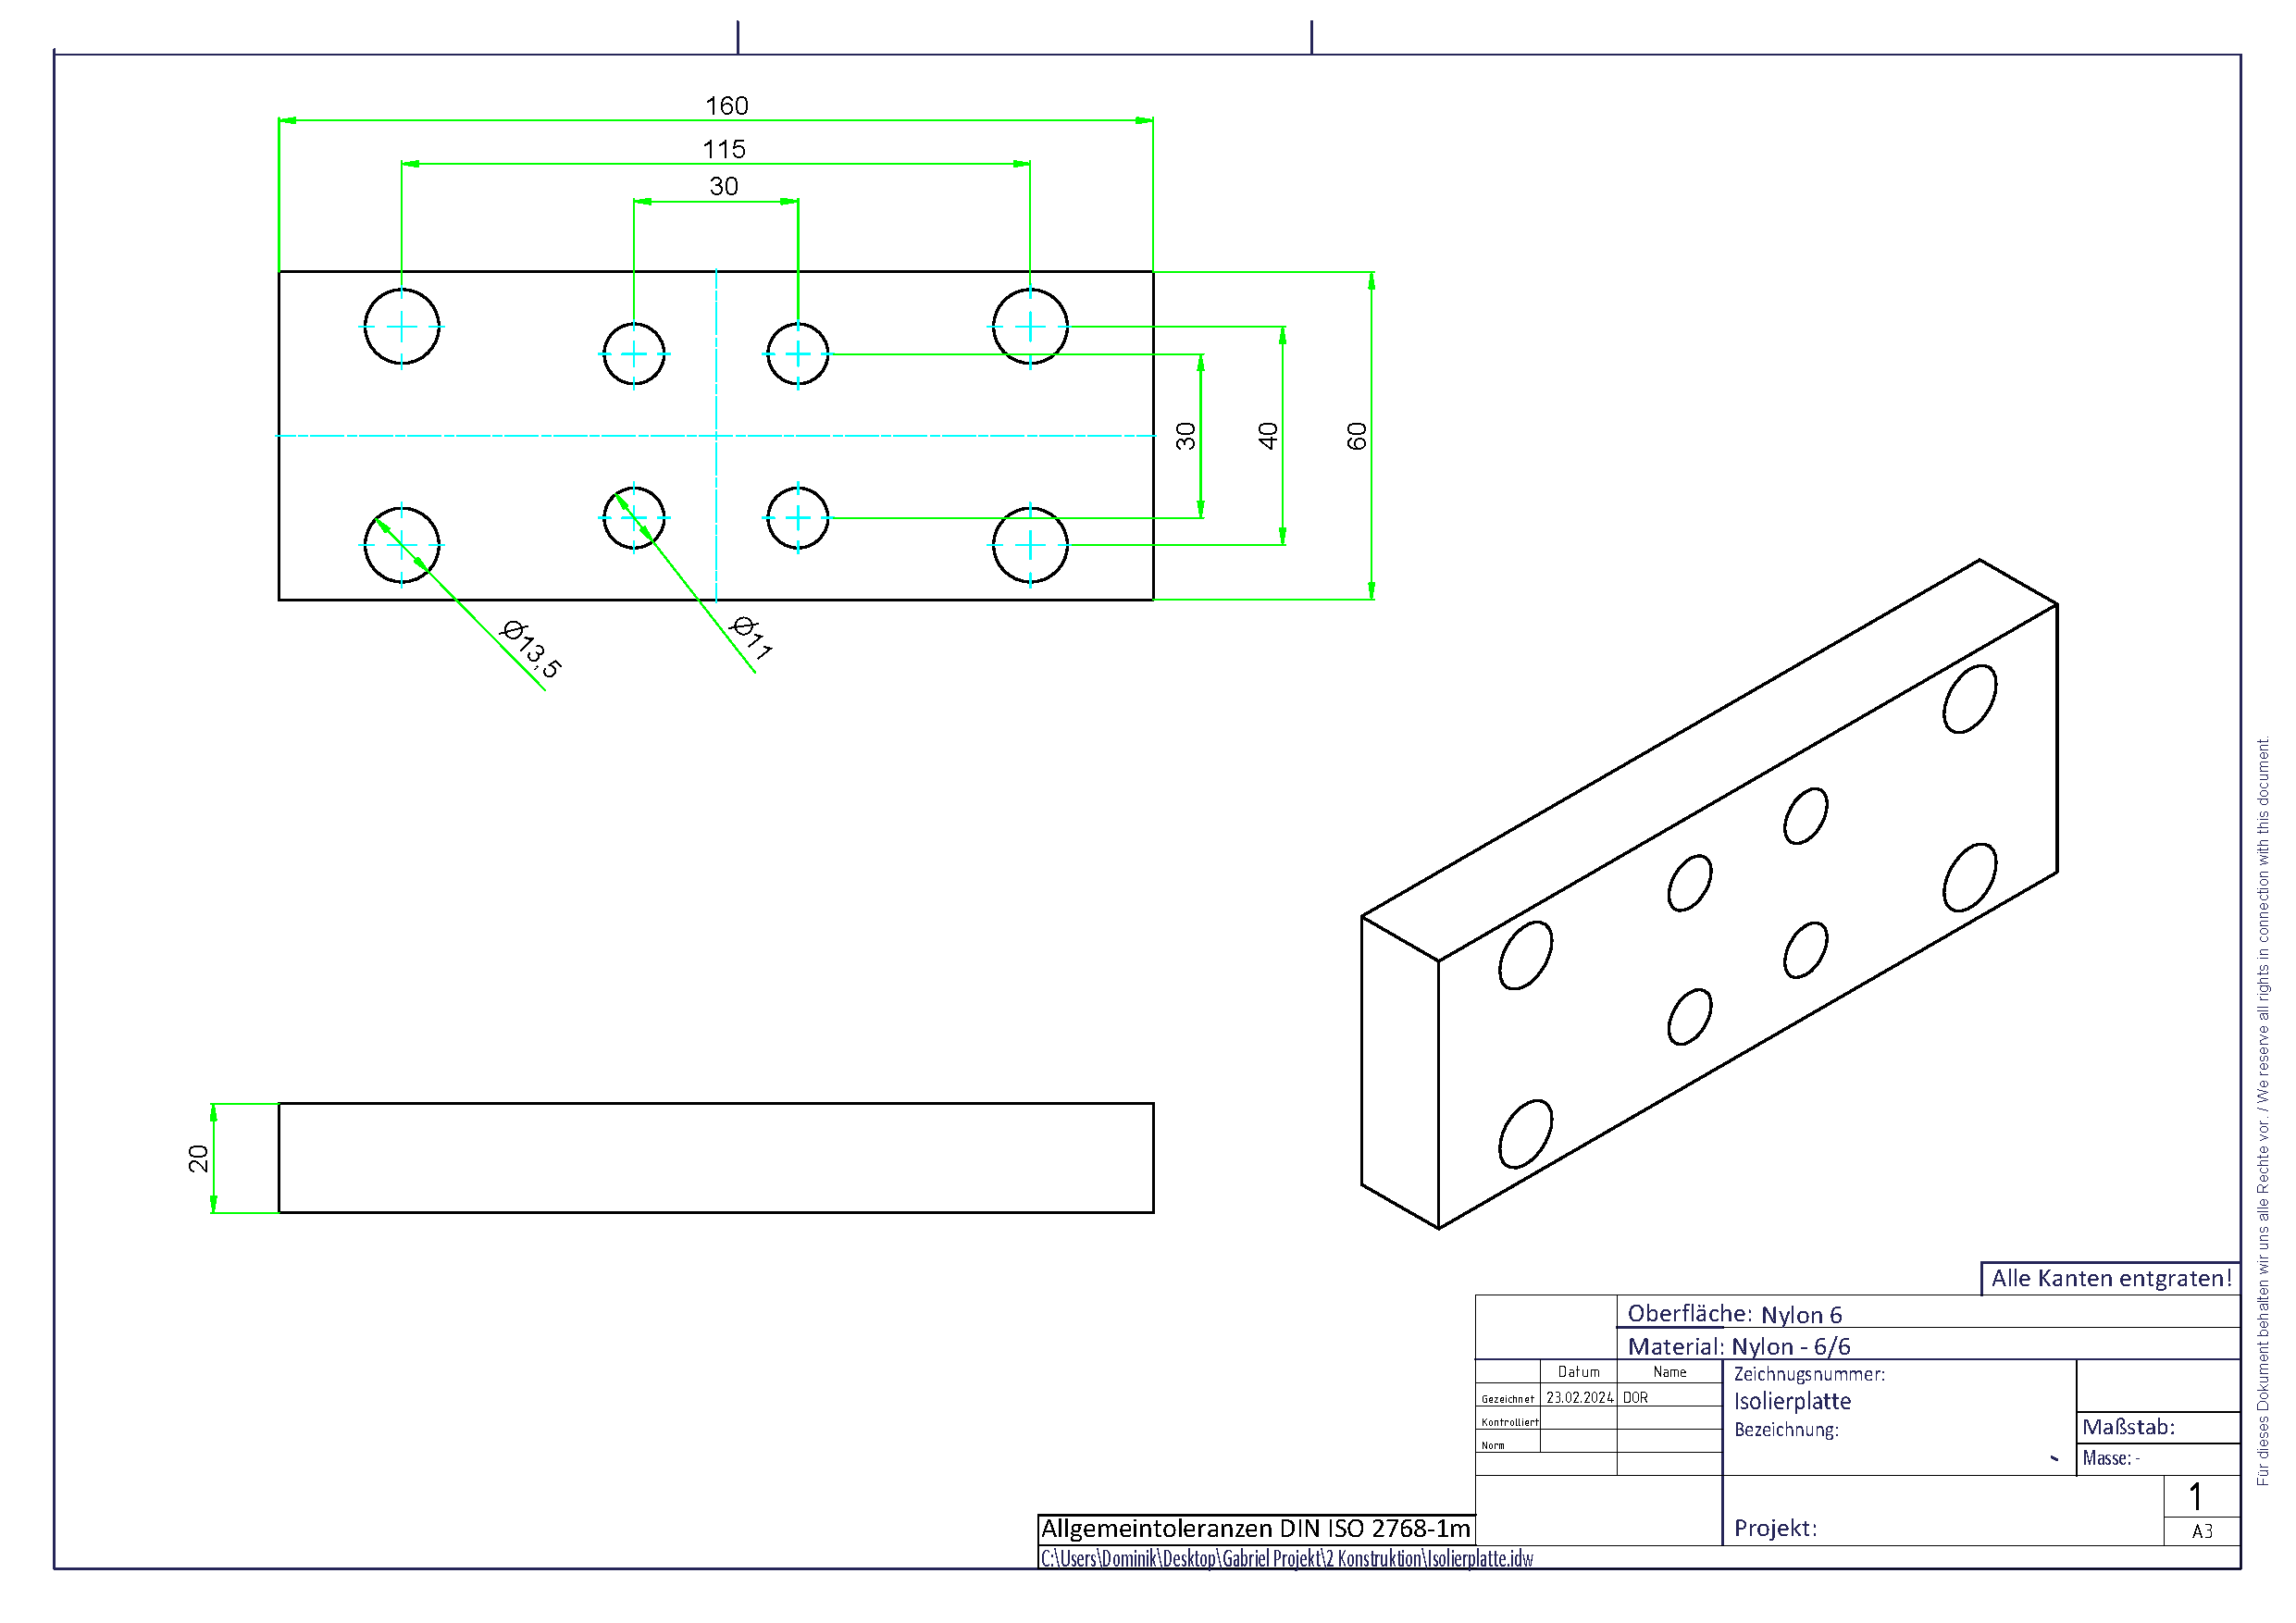
\includegraphics[angle=90,width=\textwidth]{../ref/Isolierplatte.pdf}
	\caption{Zeichnung der Teflonplatte}
	\label{fig:Teflonplatte-Zeichnung}
\end{figure}

\begin{figure}[h!]
	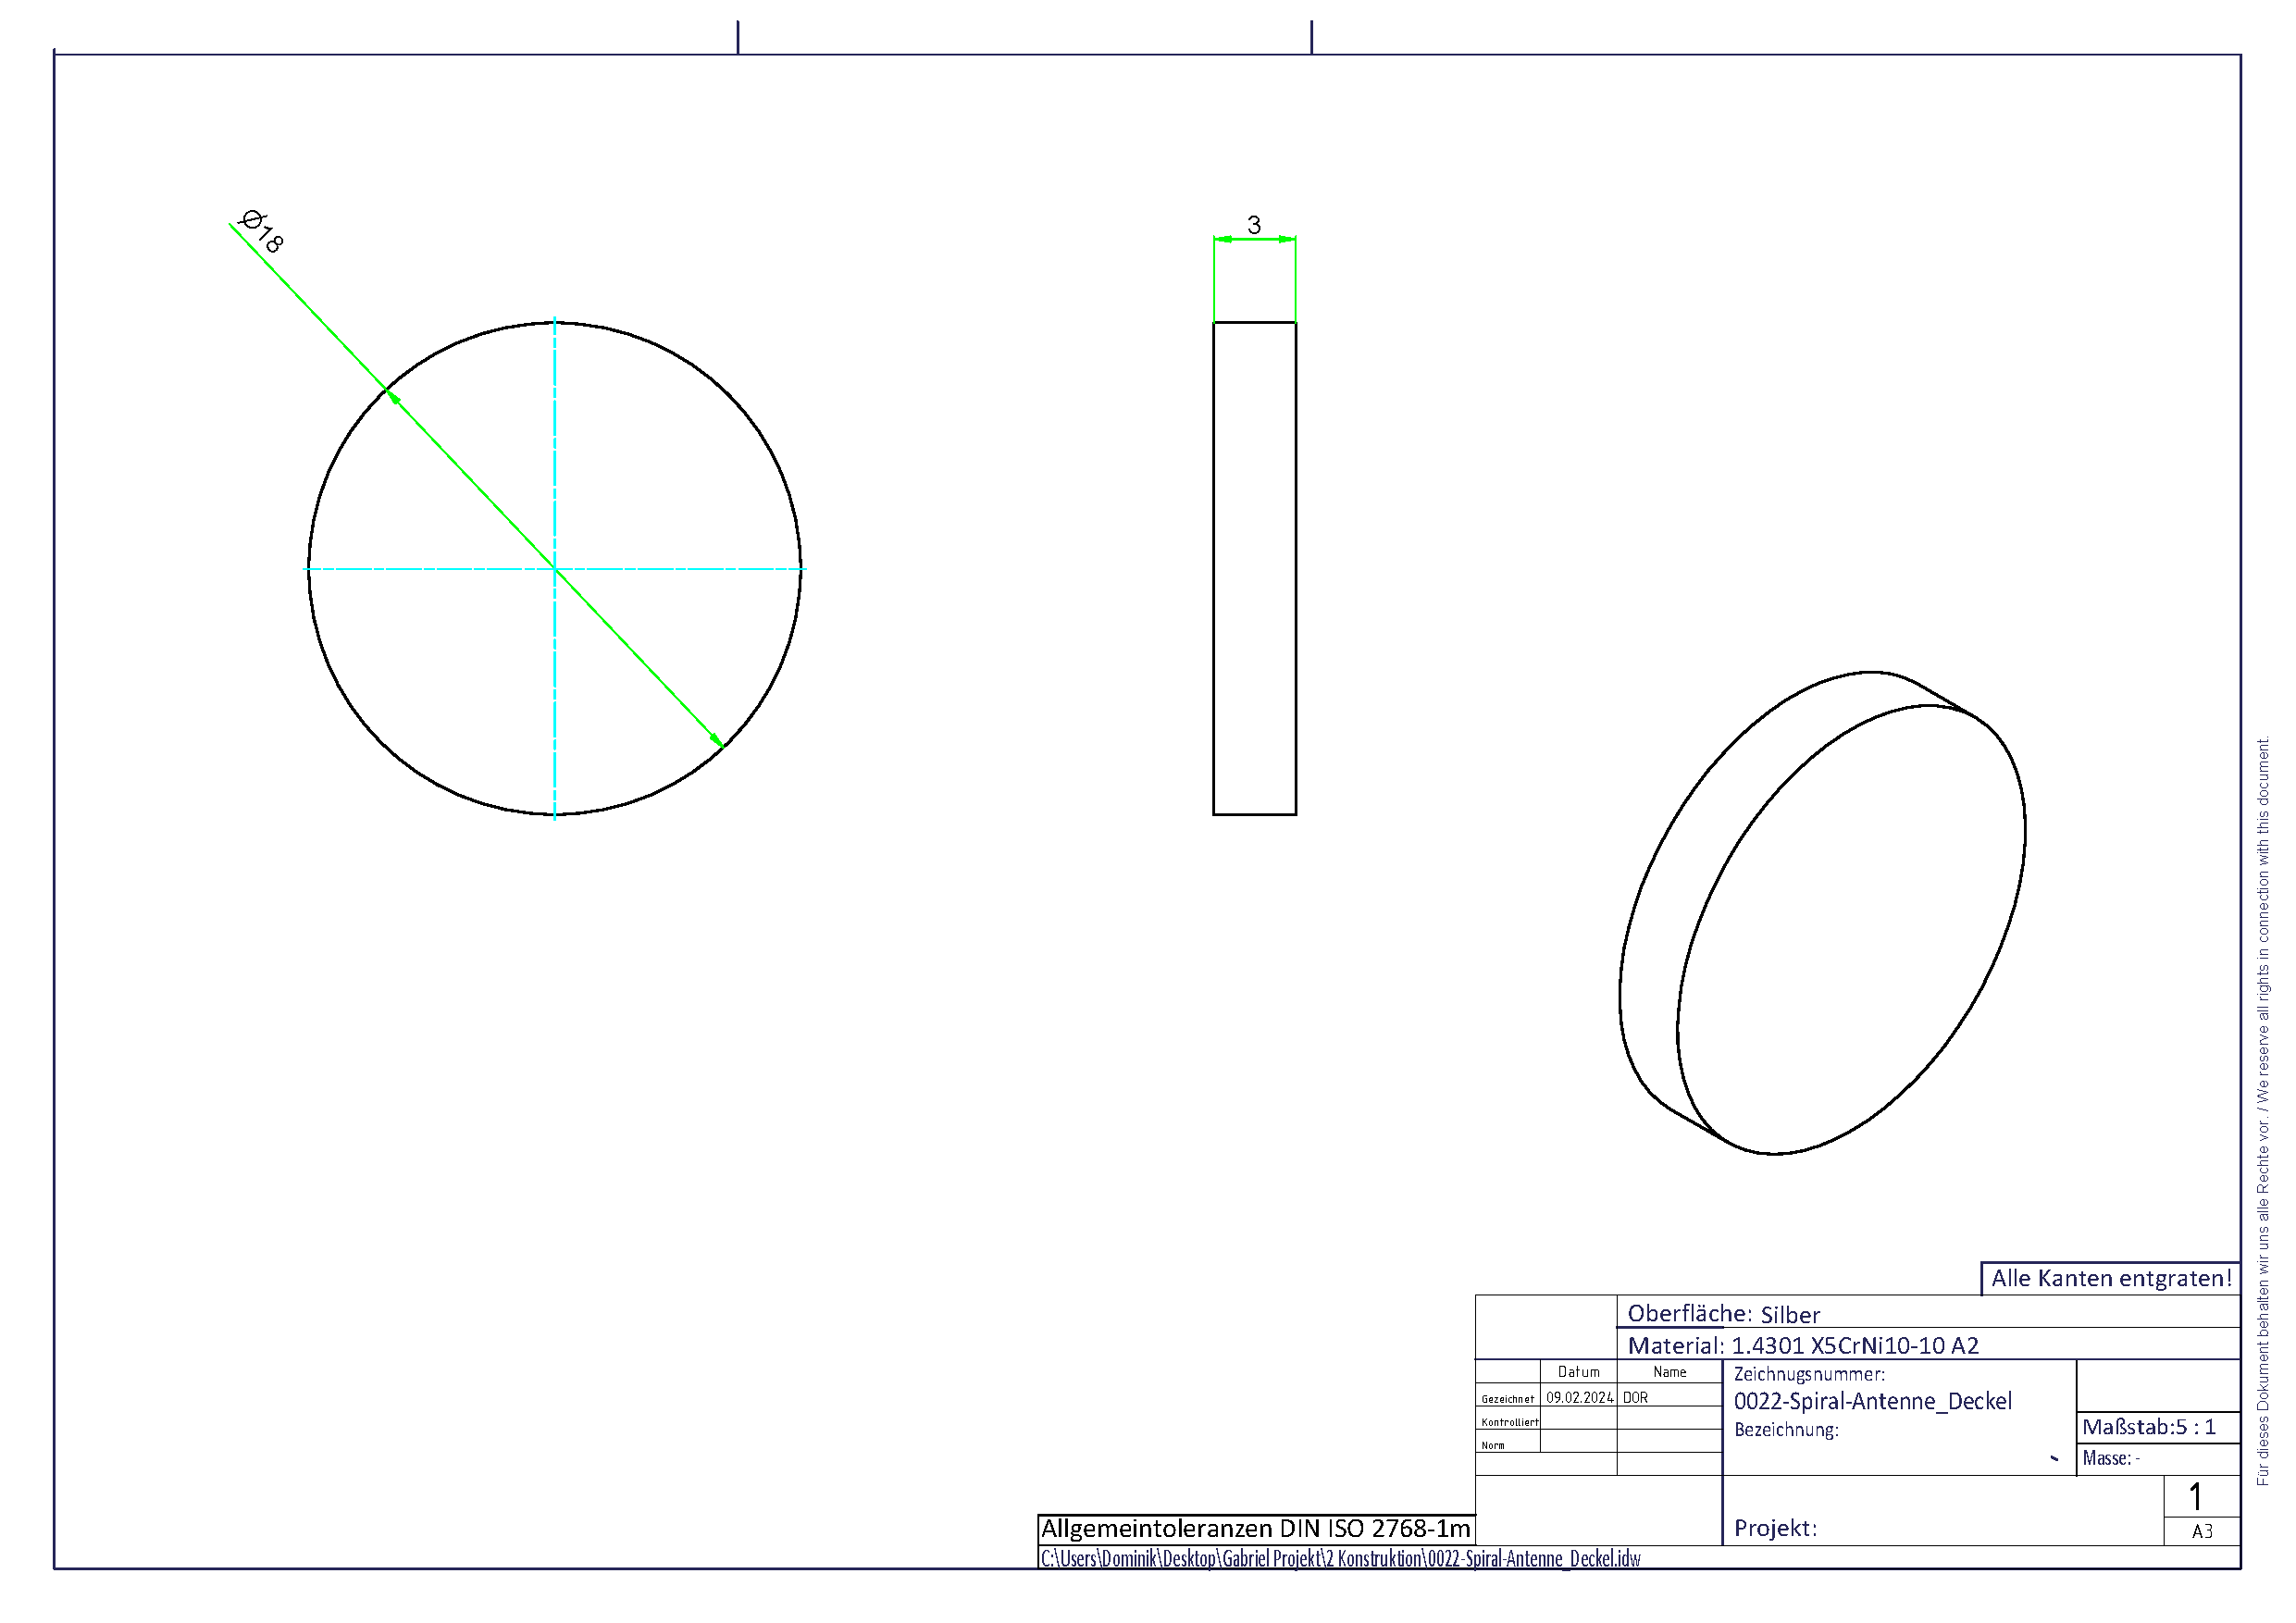
\includegraphics[angle=90,width=\textwidth]{../ref/0022-Spiral-Antenne_Deckel.pdf}
	\caption{Zeichnung des oberen Helixdeckels}
	\label{fig:Spirale-Deckel-oben}
\end{figure}

\begin{figure}[h!]
	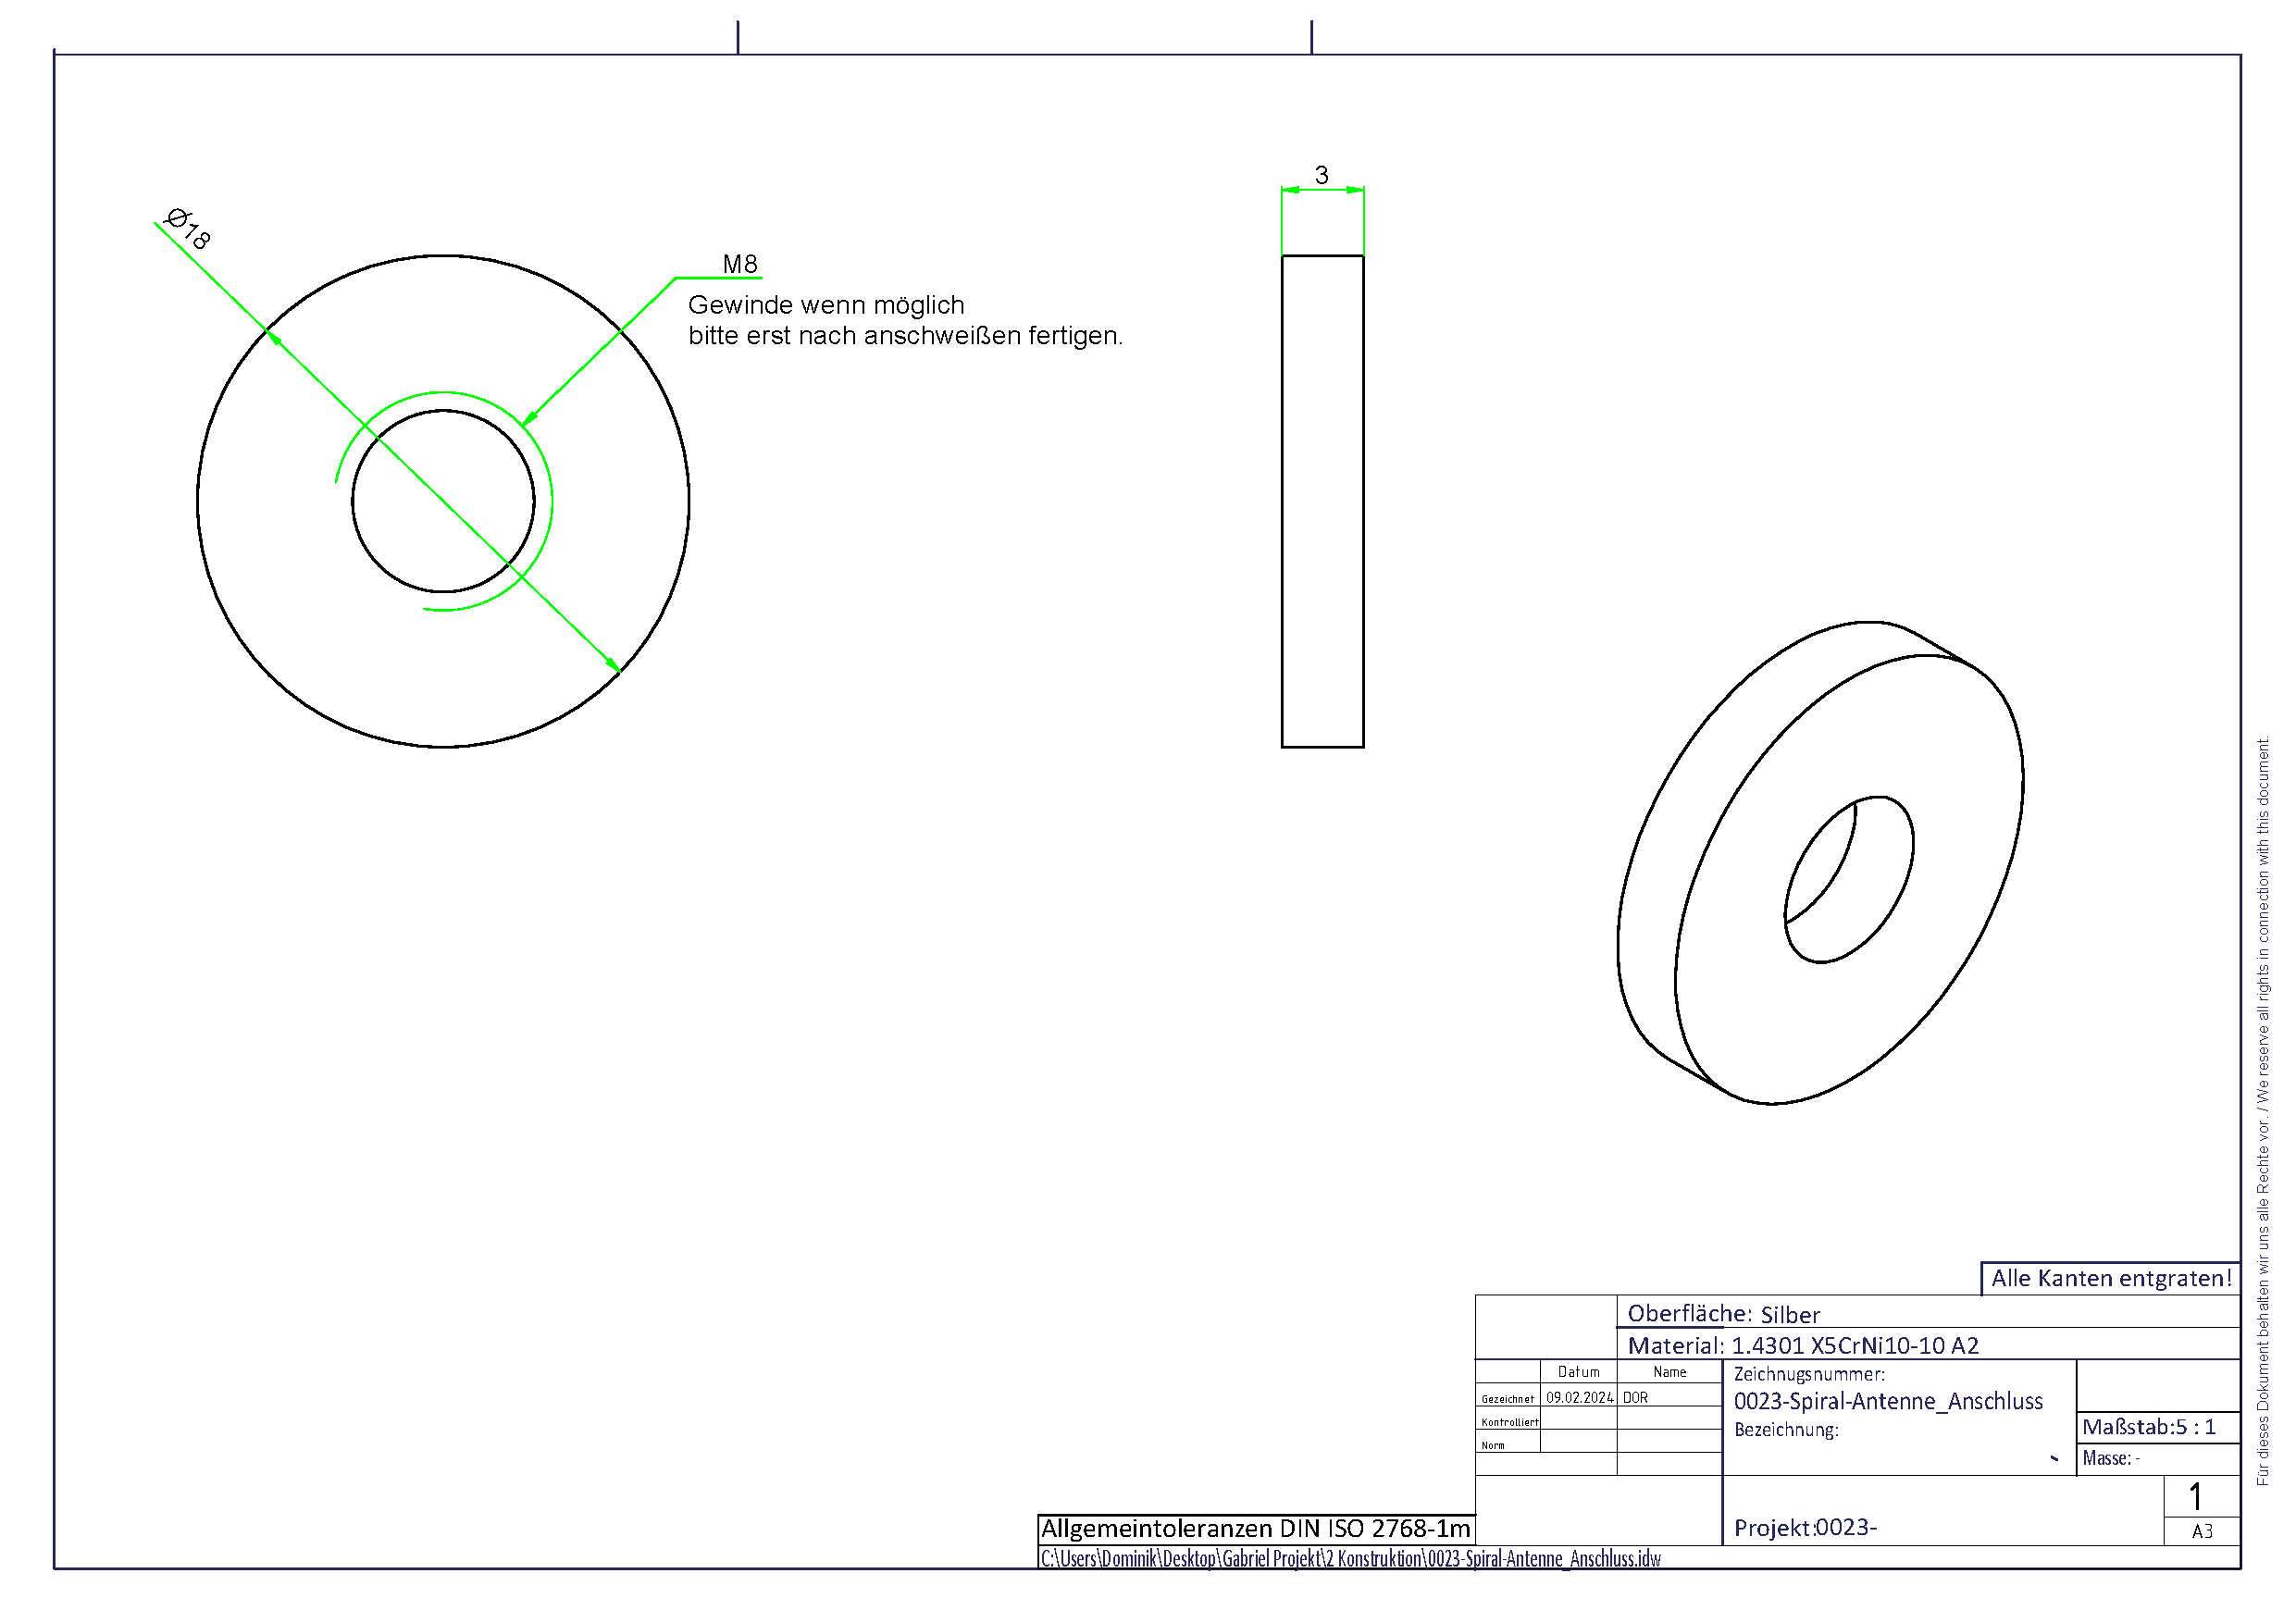
\includegraphics[angle=90,width=\textwidth]{../ref/0023-Spiral-Antenne_Anschluss.pdf}
	\caption{Zeichnung des unteren Helixdeckels}
	\label{fig:Spirale-Deckel-unten}
\end{figure}

\begin{figure}[h!]
	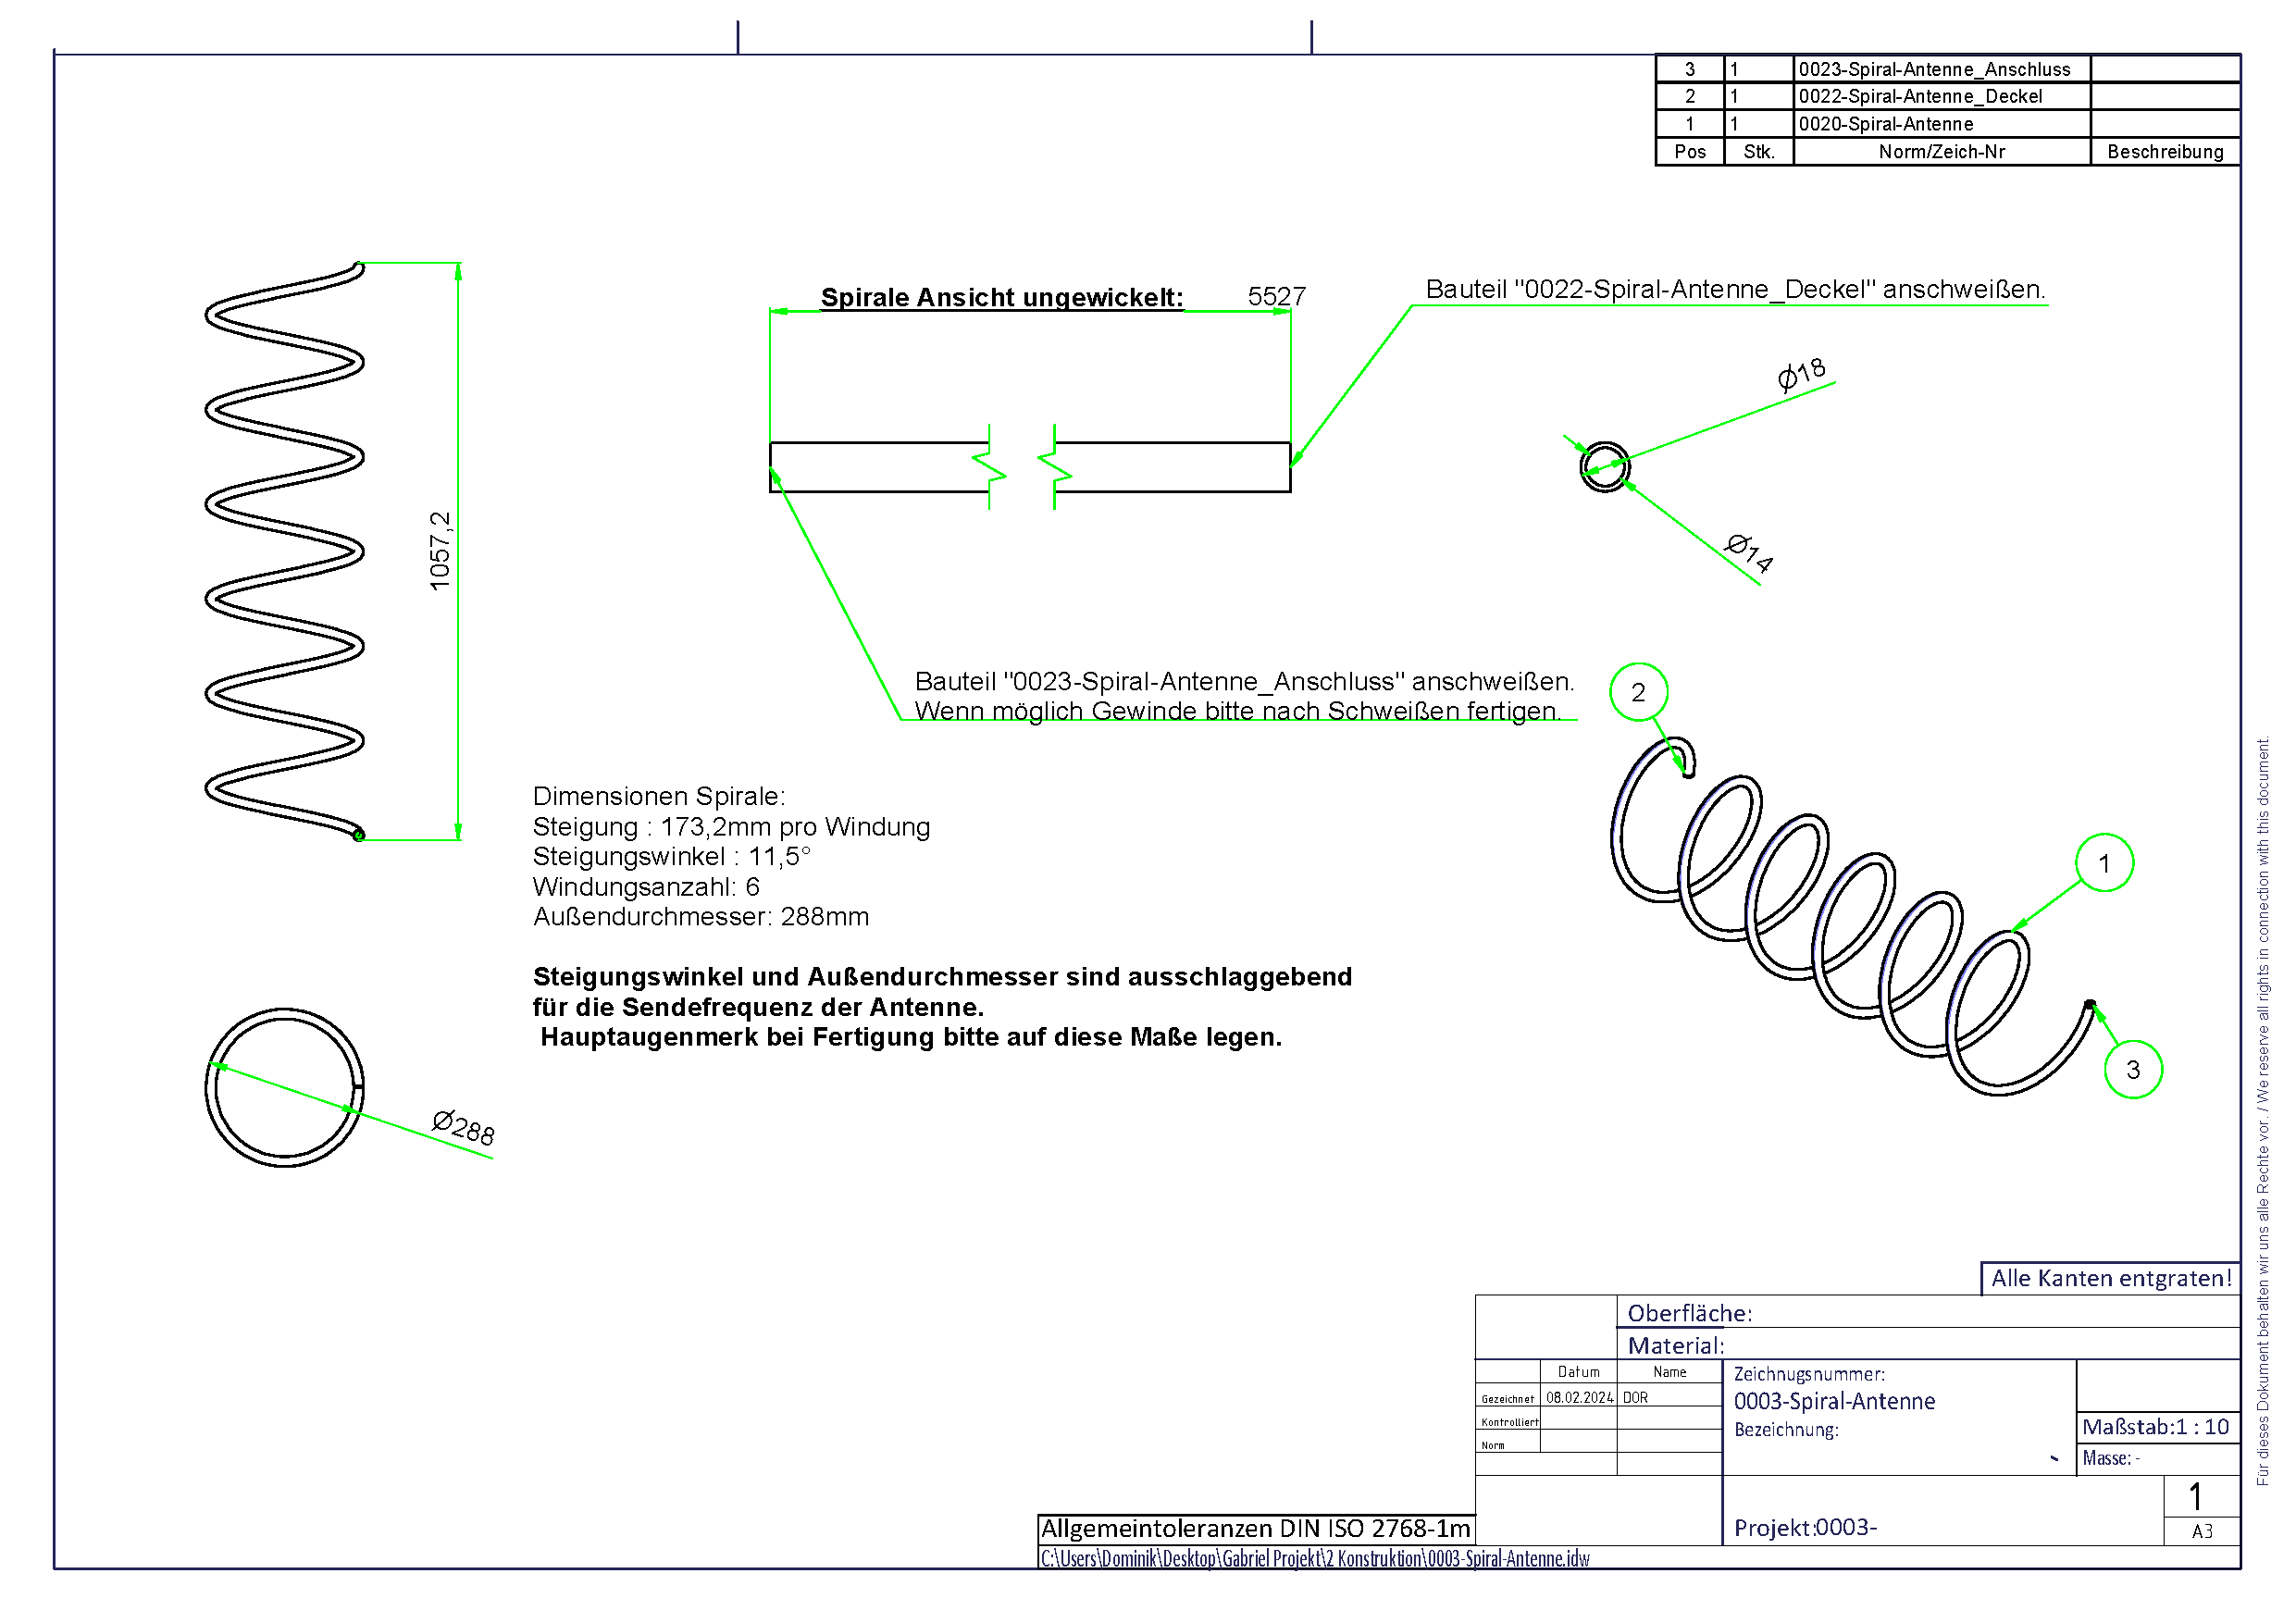
\includegraphics[angle=90,width=\textwidth]{../ref/0003-Spiral-Antenne.pdf}
	\caption{Zeichnung der Spirale der Helixantenne}
	\label{fig:Spirale-Antenne}
\end{figure}

\begin{figure}[h!]
	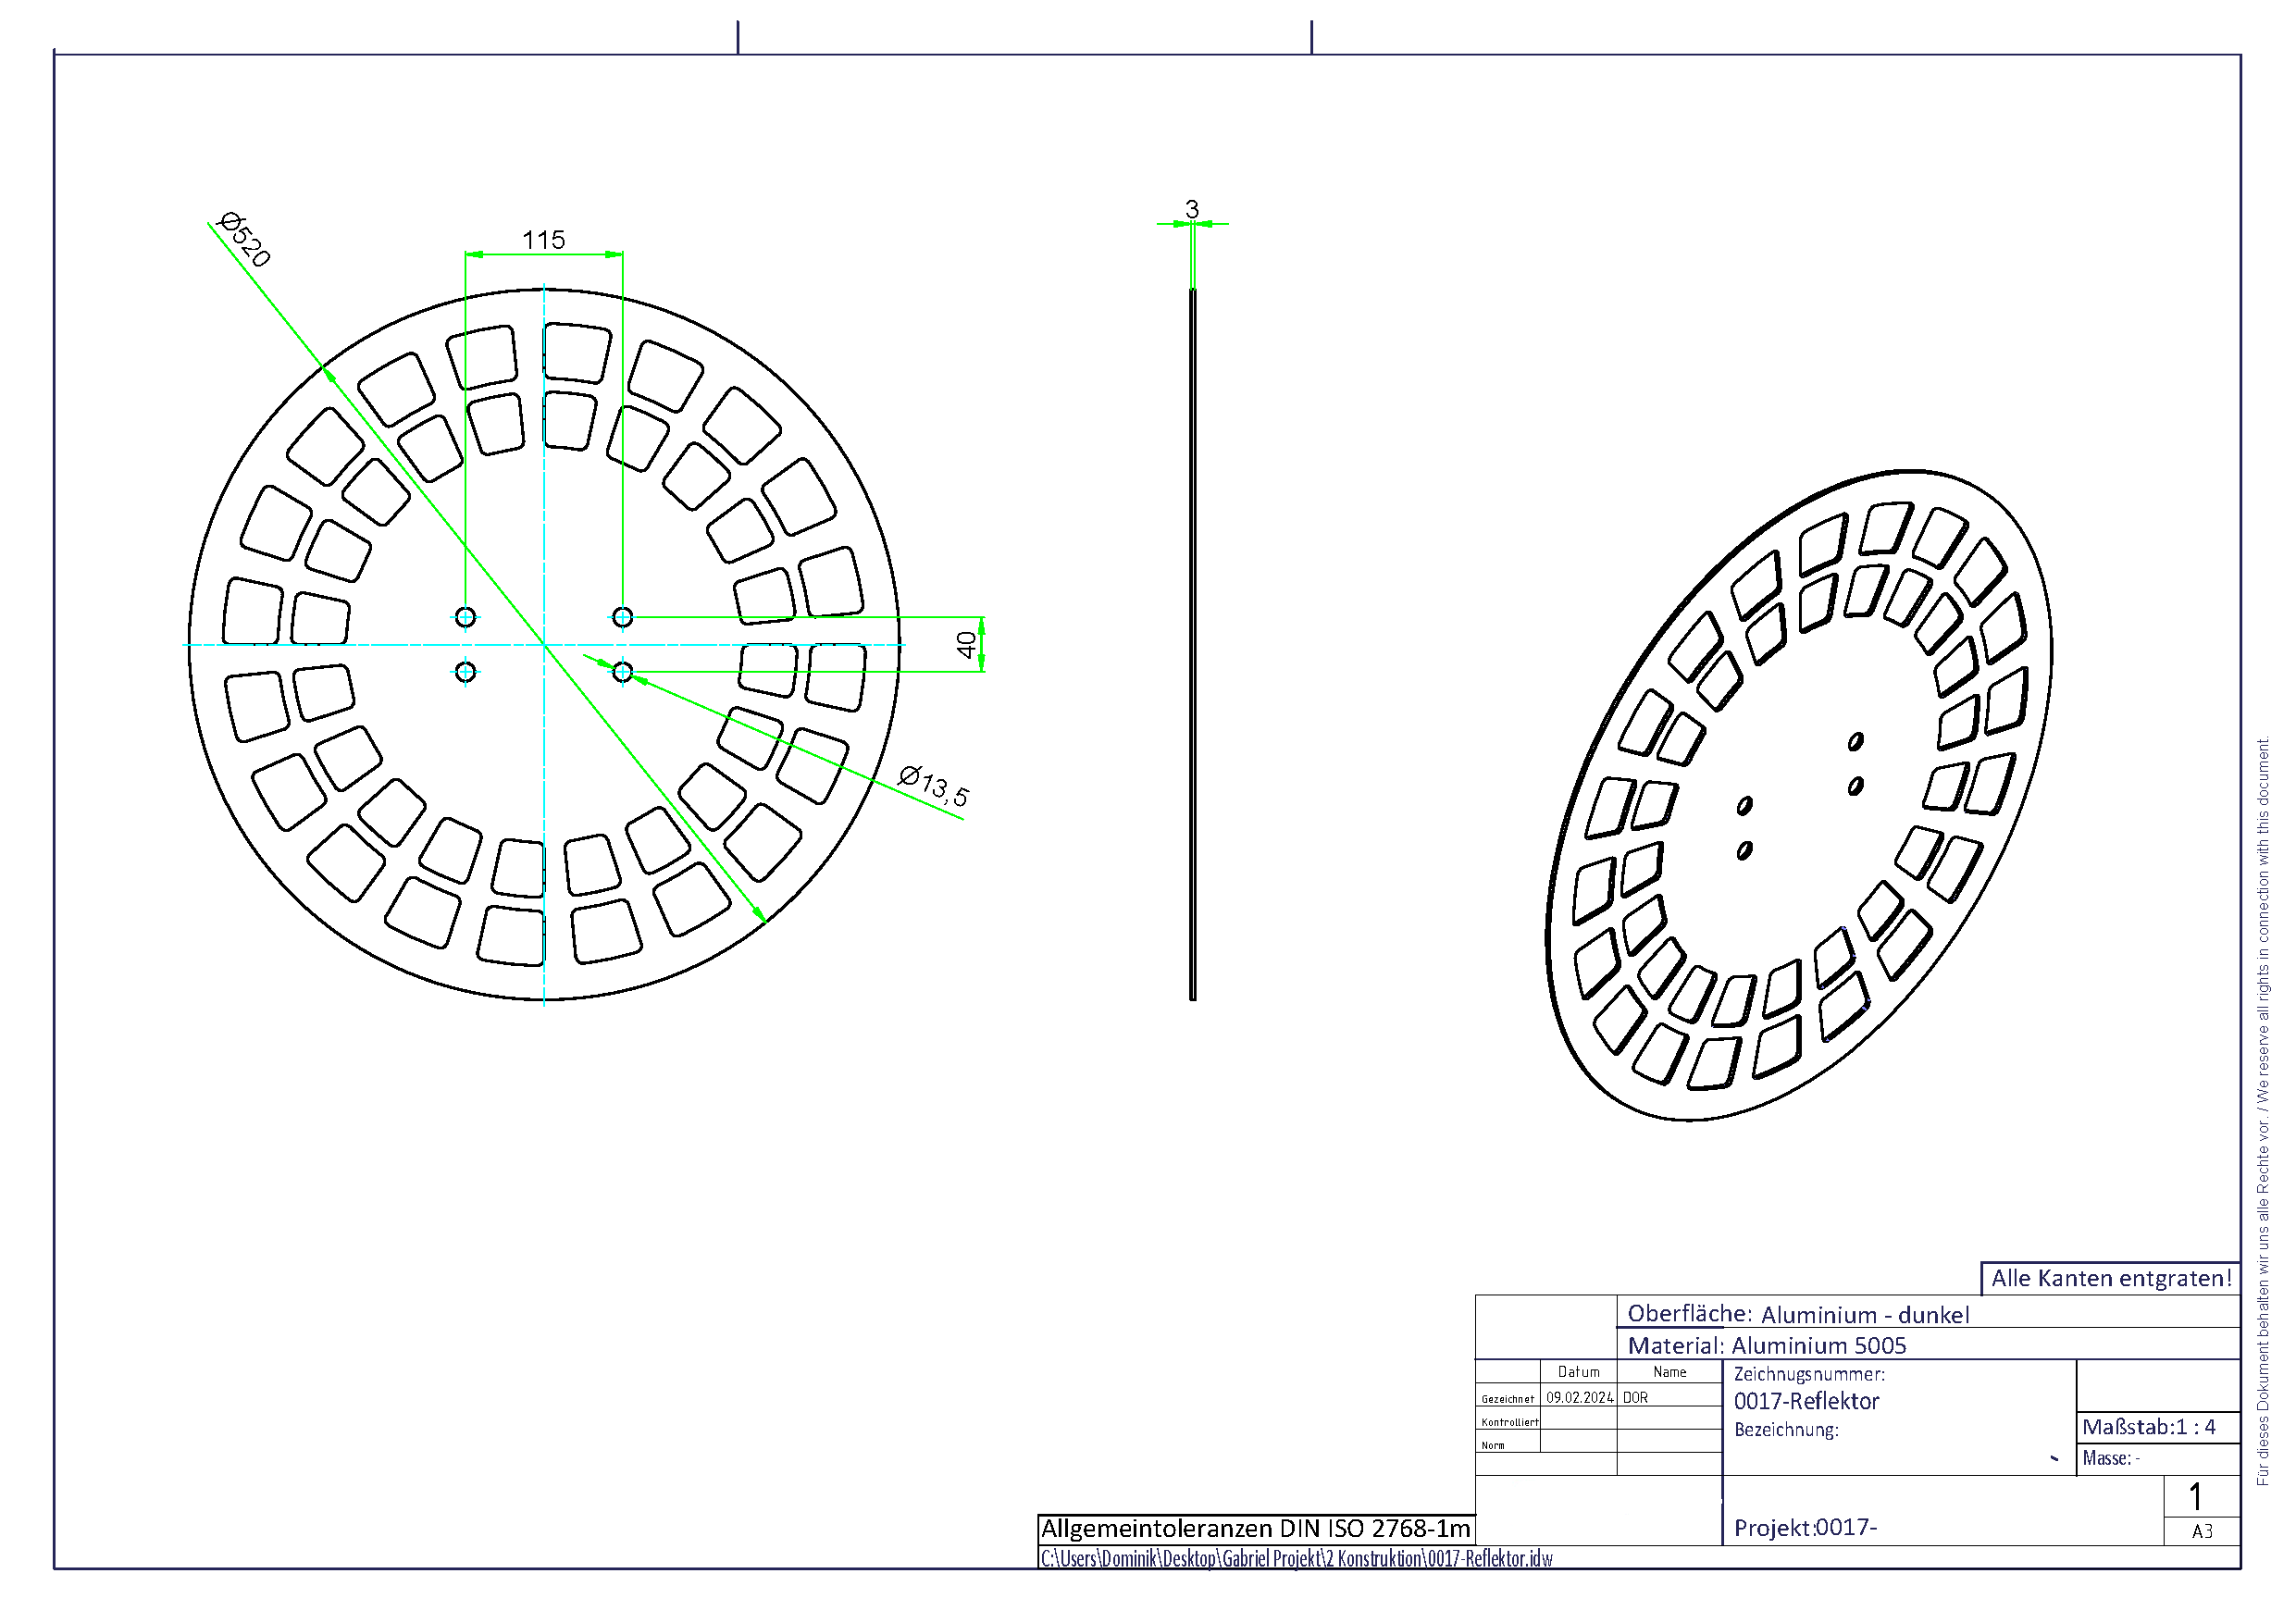
\includegraphics[angle=90,width=\textwidth]{../ref/0017-Reflektor.pdf}
	\caption{Zeichnung des Reflektors}
	\label{fig:Reflektor-Zeichnung}
\end{figure}

\begin{figure}[h!]
	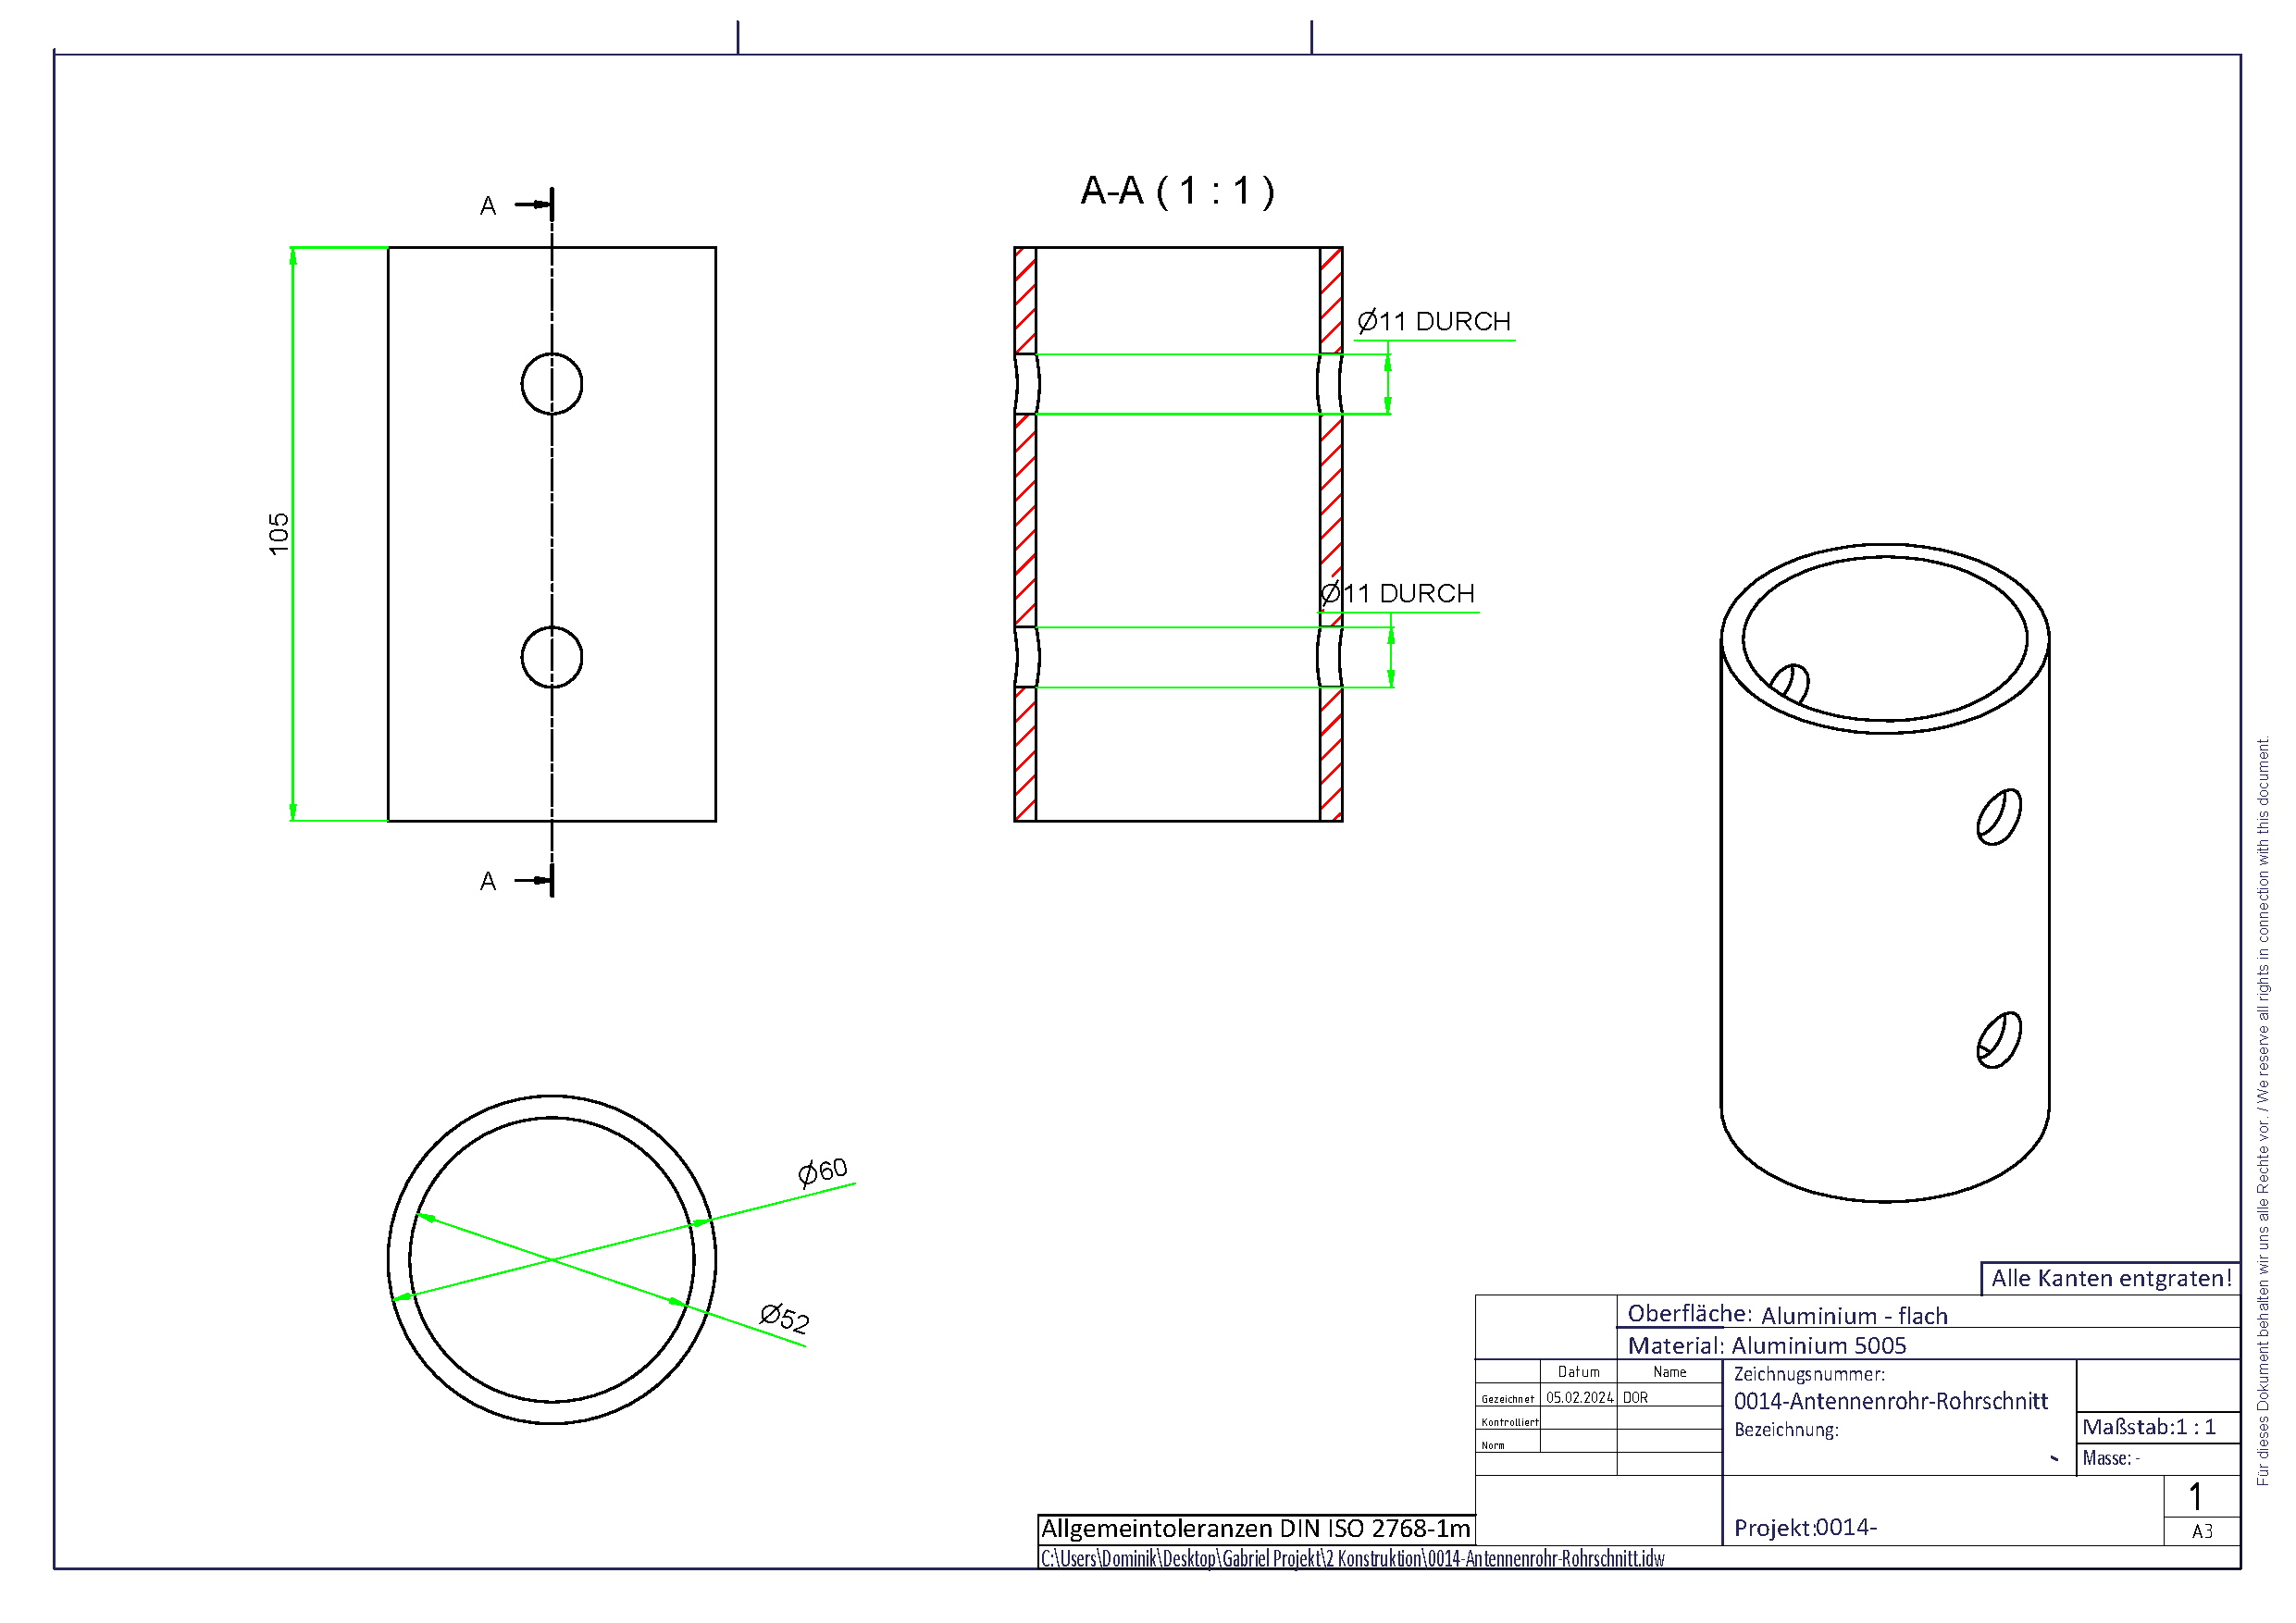
\includegraphics[angle=90,width=\textwidth]{../ref/0014-Antennenrohr-Rohrschnitt.pdf}
	\caption{Zeichnung des Rohrschnitts des Antennen-Rohrflansches}
	\label{fig:Rohrschnitt-Rohrflansch-Antenne}
\end{figure}

\begin{figure}[h!]
	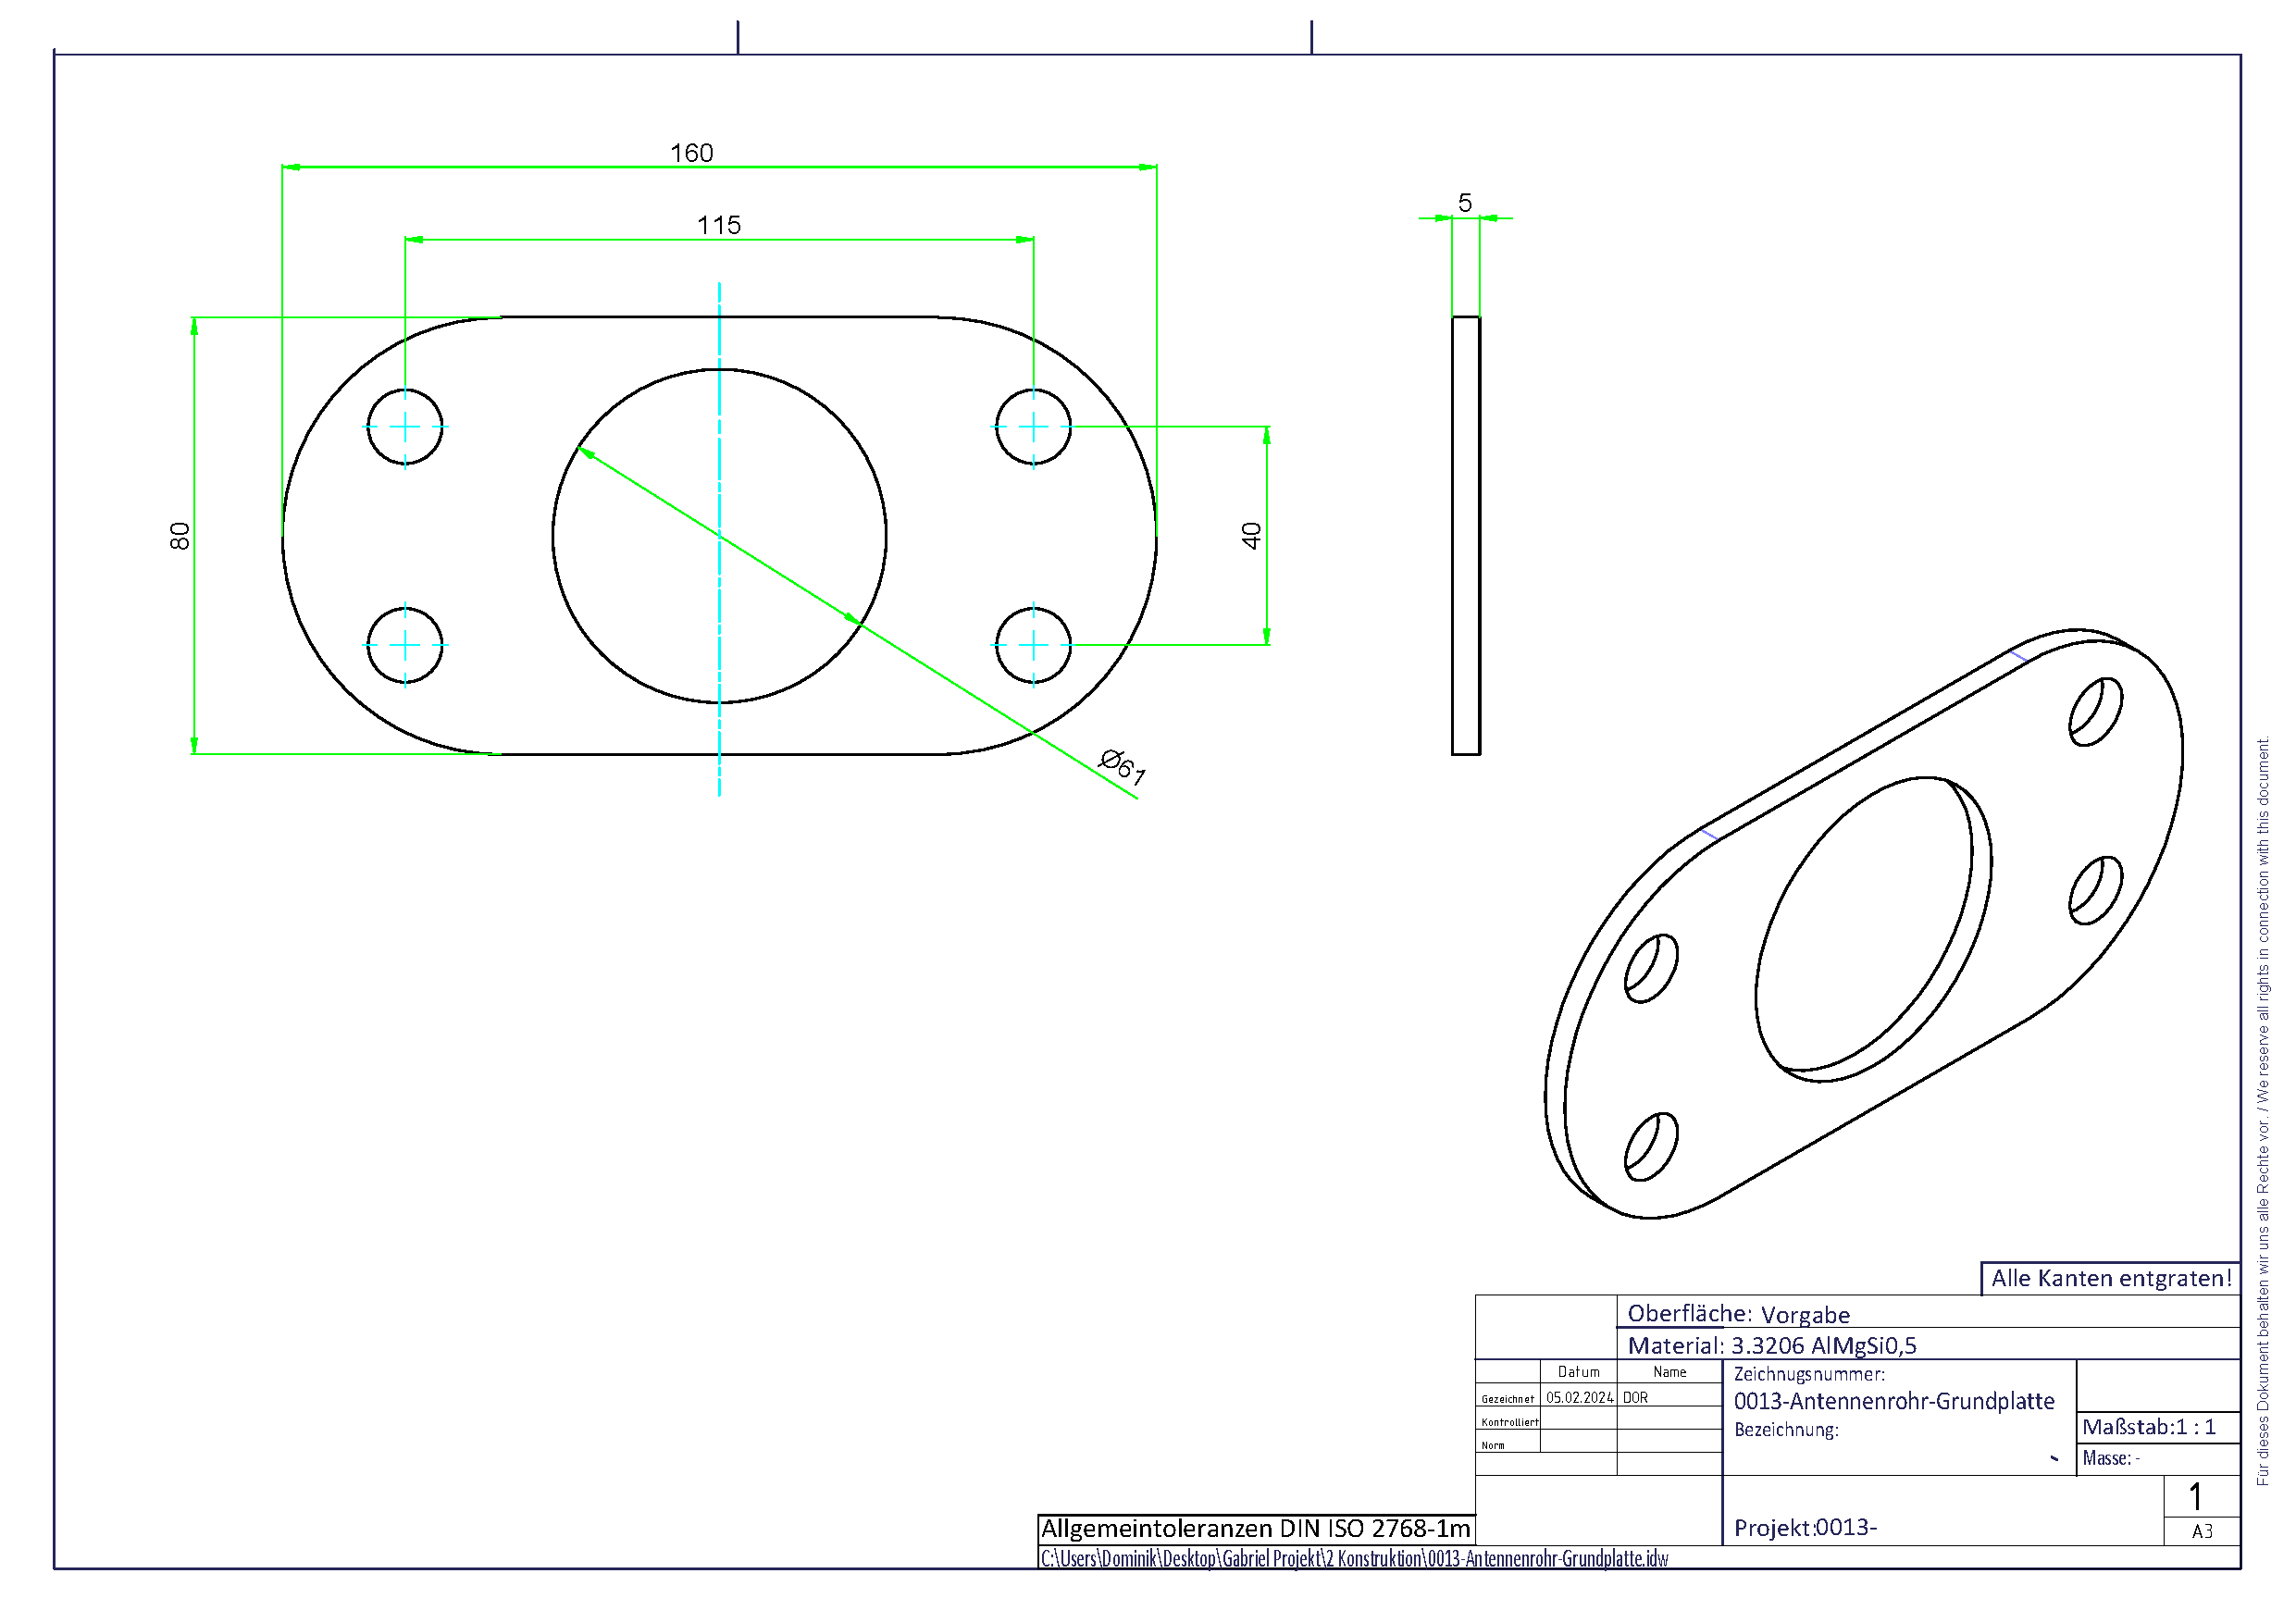
\includegraphics[angle=90,width=\textwidth]{../ref/0013-Antennenrohr-Grundplatte.pdf}
	\caption{Zeichnung der Grundplatte des Antennen-Rohrflansches}
	\label{fig:Grundplattelatte-Rohrflansch-Antenne}
\end{figure}

\begin{figure}[h!]
	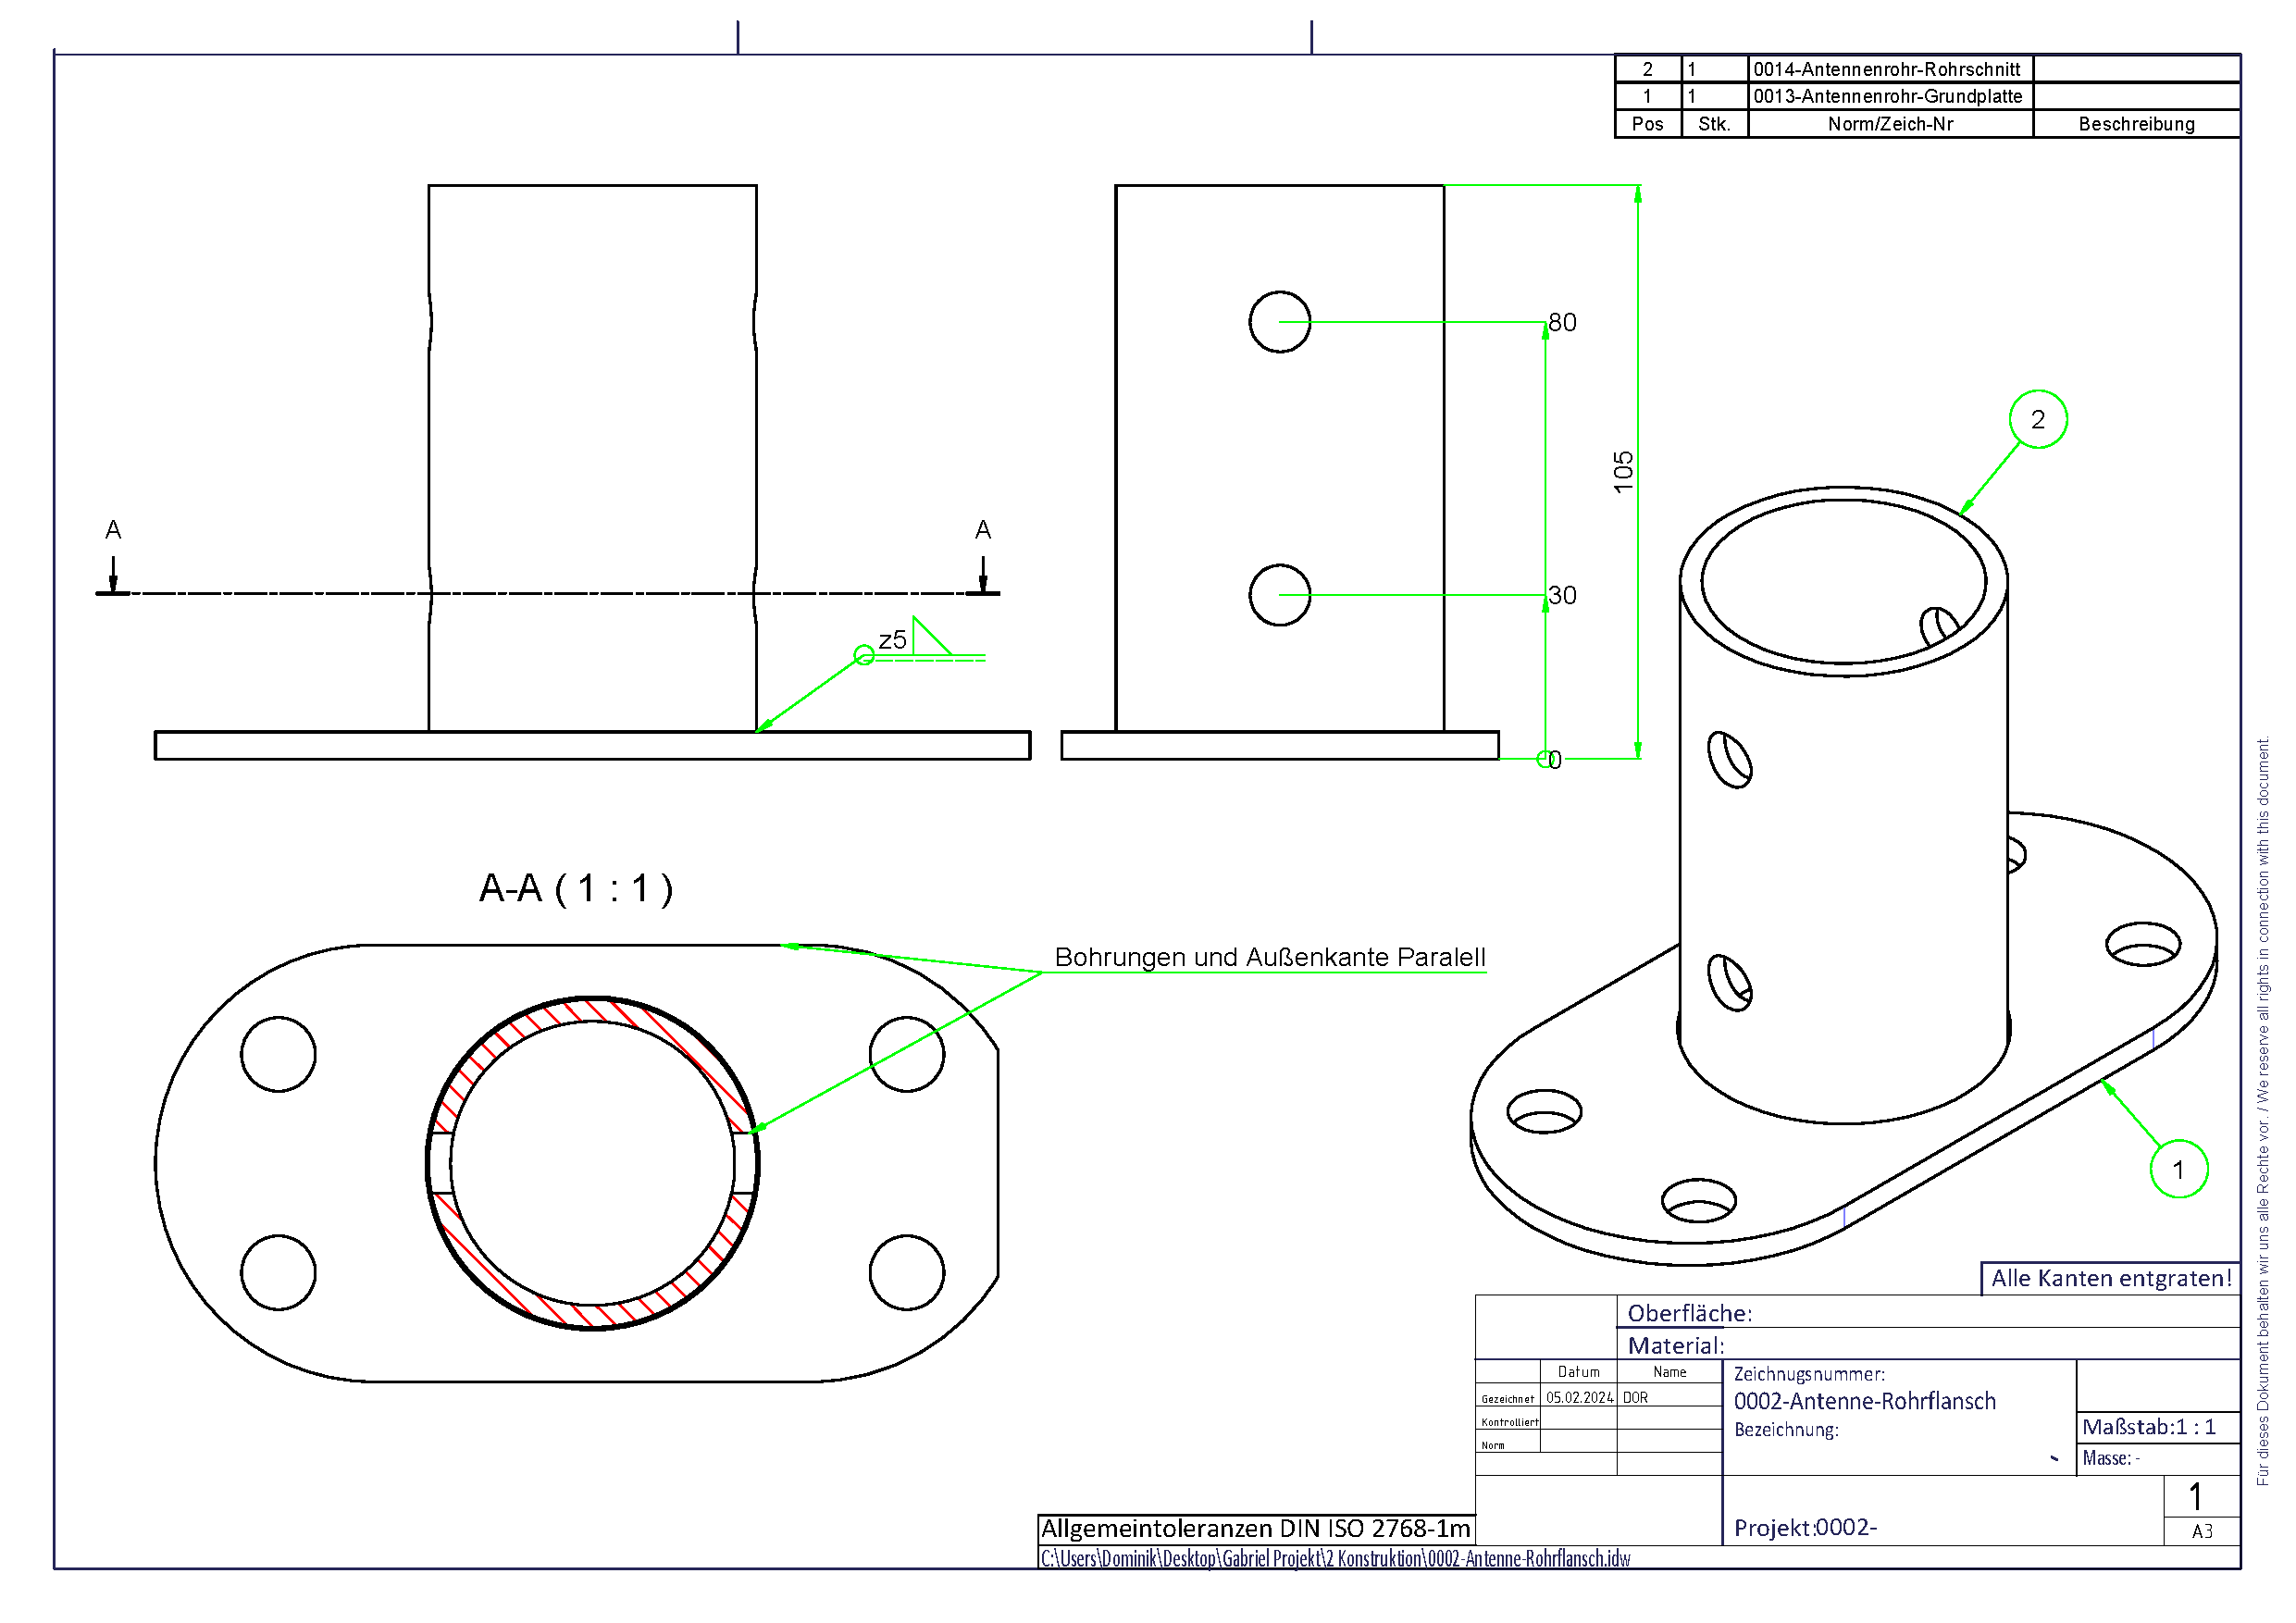
\includegraphics[angle=90,width=\textwidth]{../ref/0002-Antenne-Rohrflansch.pdf}
	\caption{Zeichnung des Antennen-Rohrflansches}
	\label{fig:Rohrflansch-Antenne}
\end{figure}

\begin{figure}[h!]
	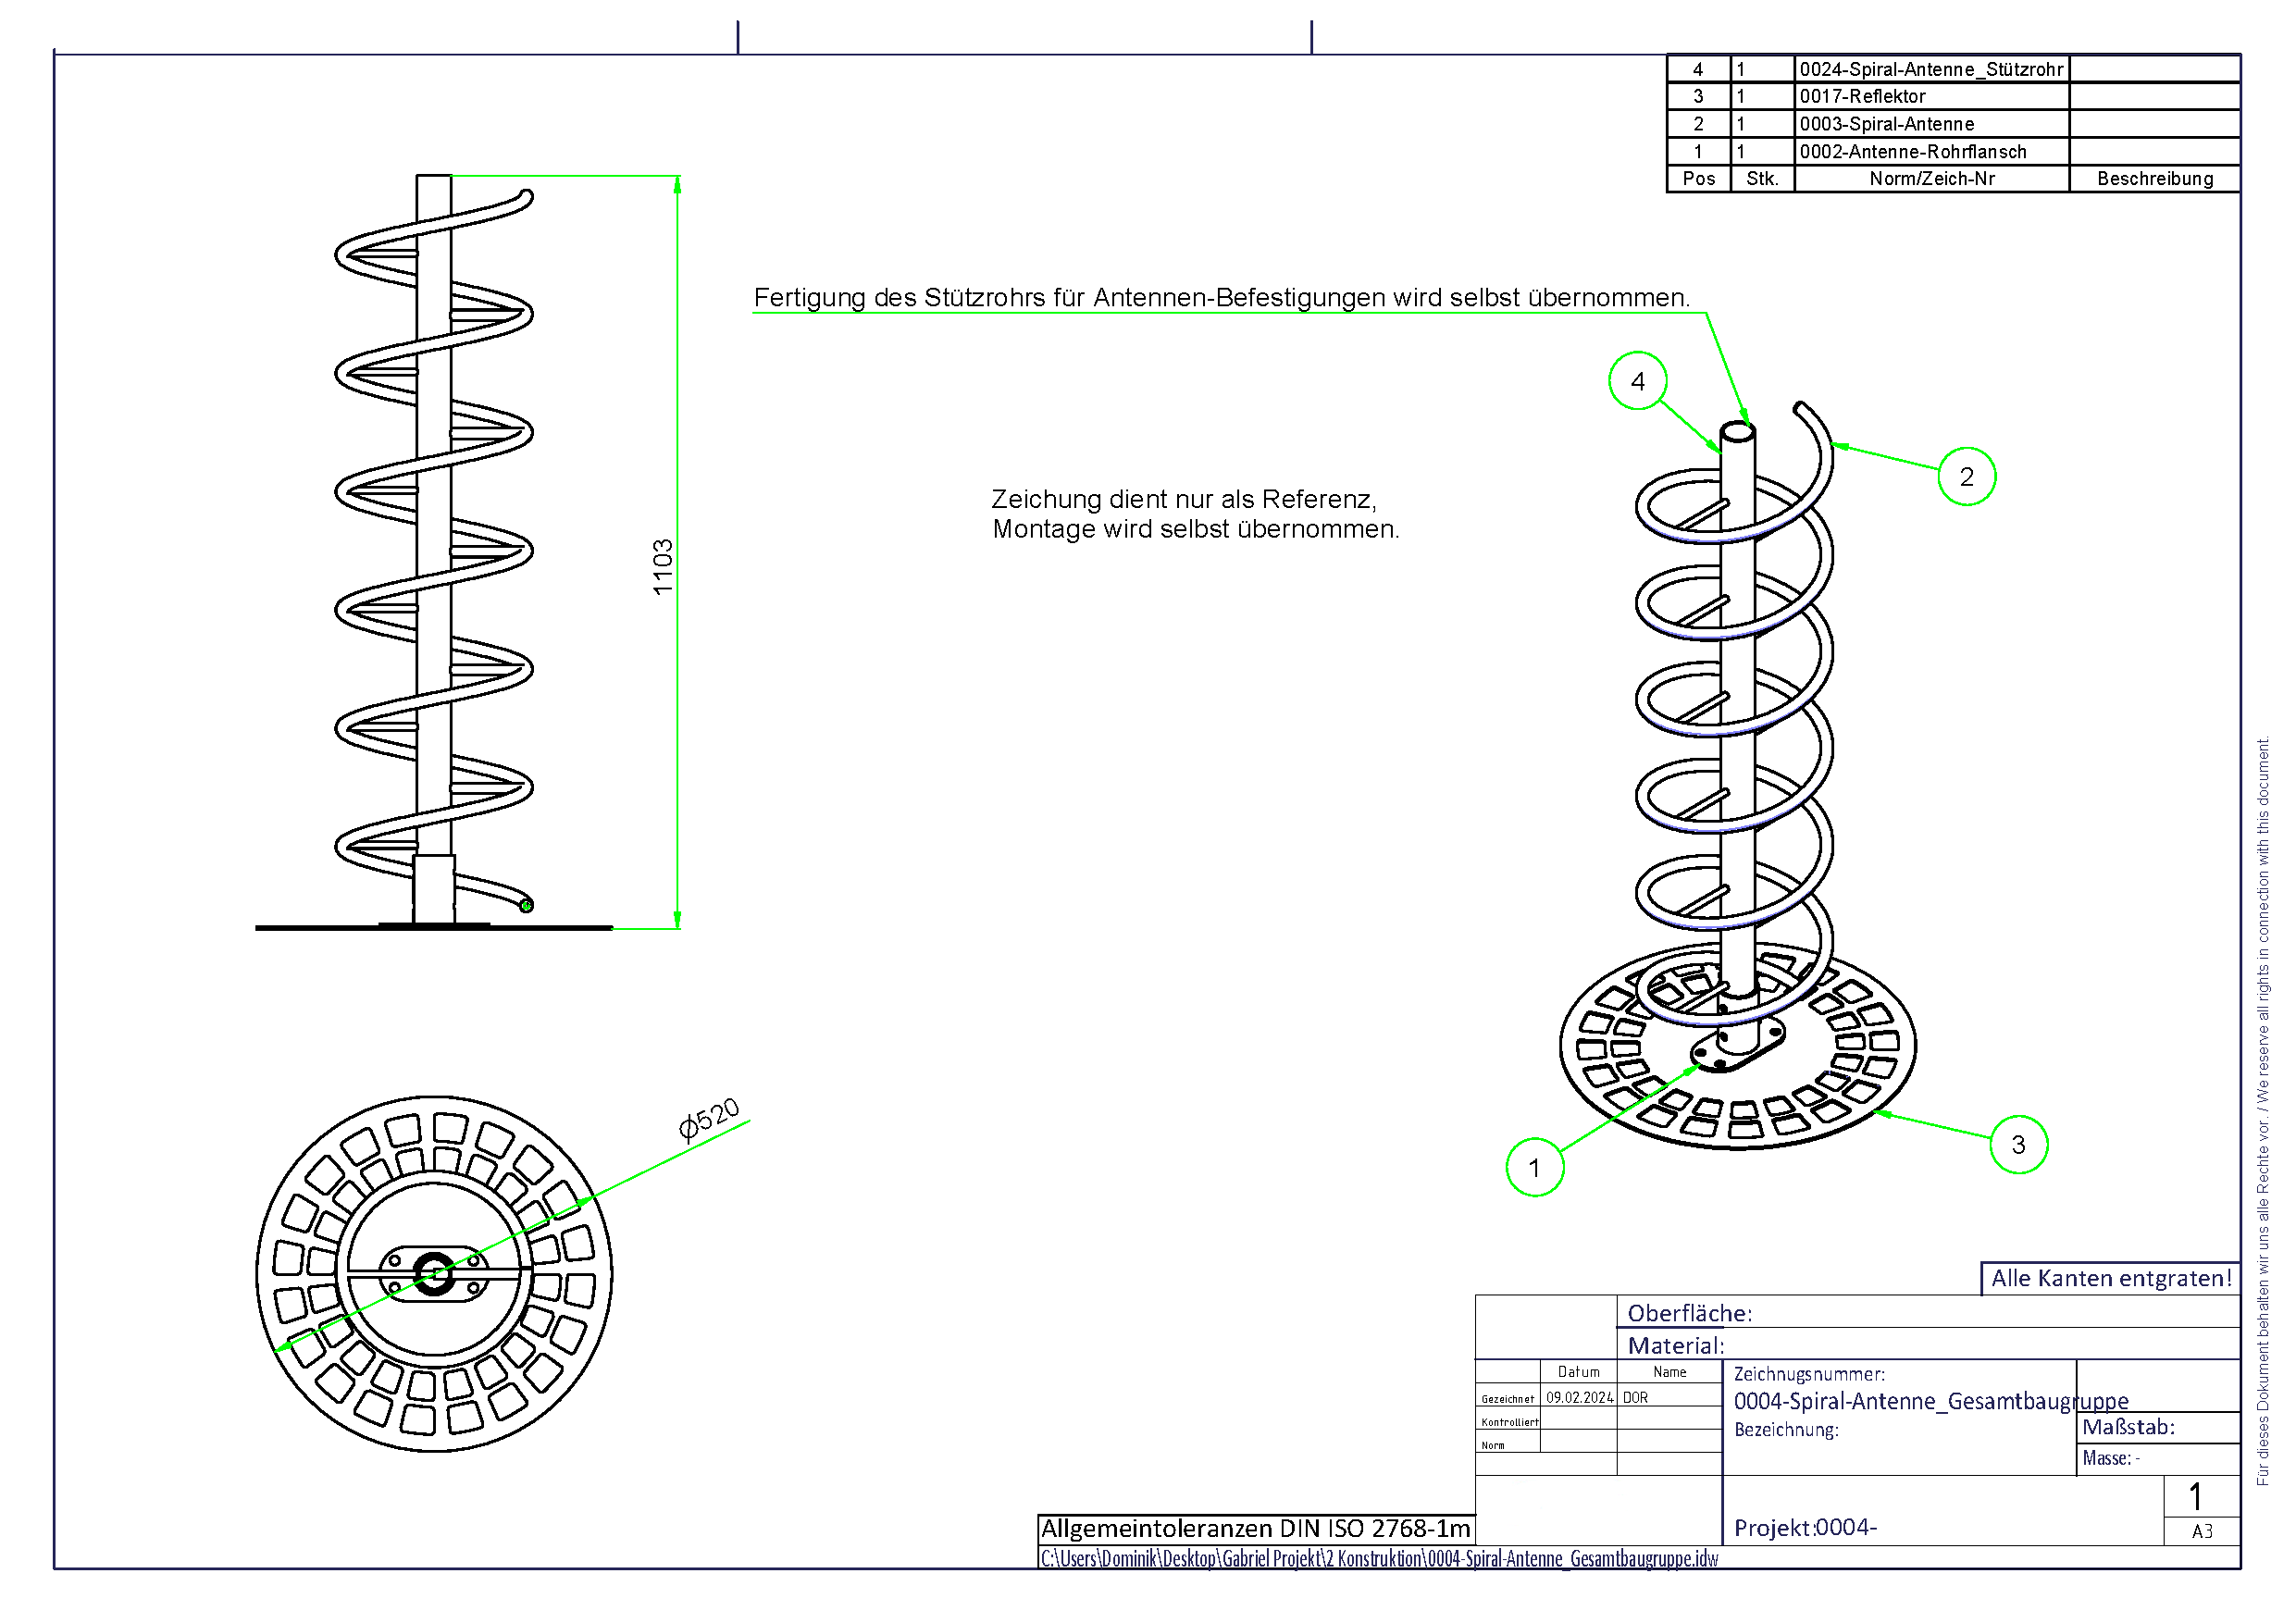
\includegraphics[angle=90,width=\textwidth]{../ref/0004-Spiral-Antenne_Gesamtbaugruppe.pdf}
	\caption{Zeichnung der Helixantennen Baugruppe}
	\label{fig:Zeichnung der Helixantenne}
\end{figure}

\begin{figure}[h!]
	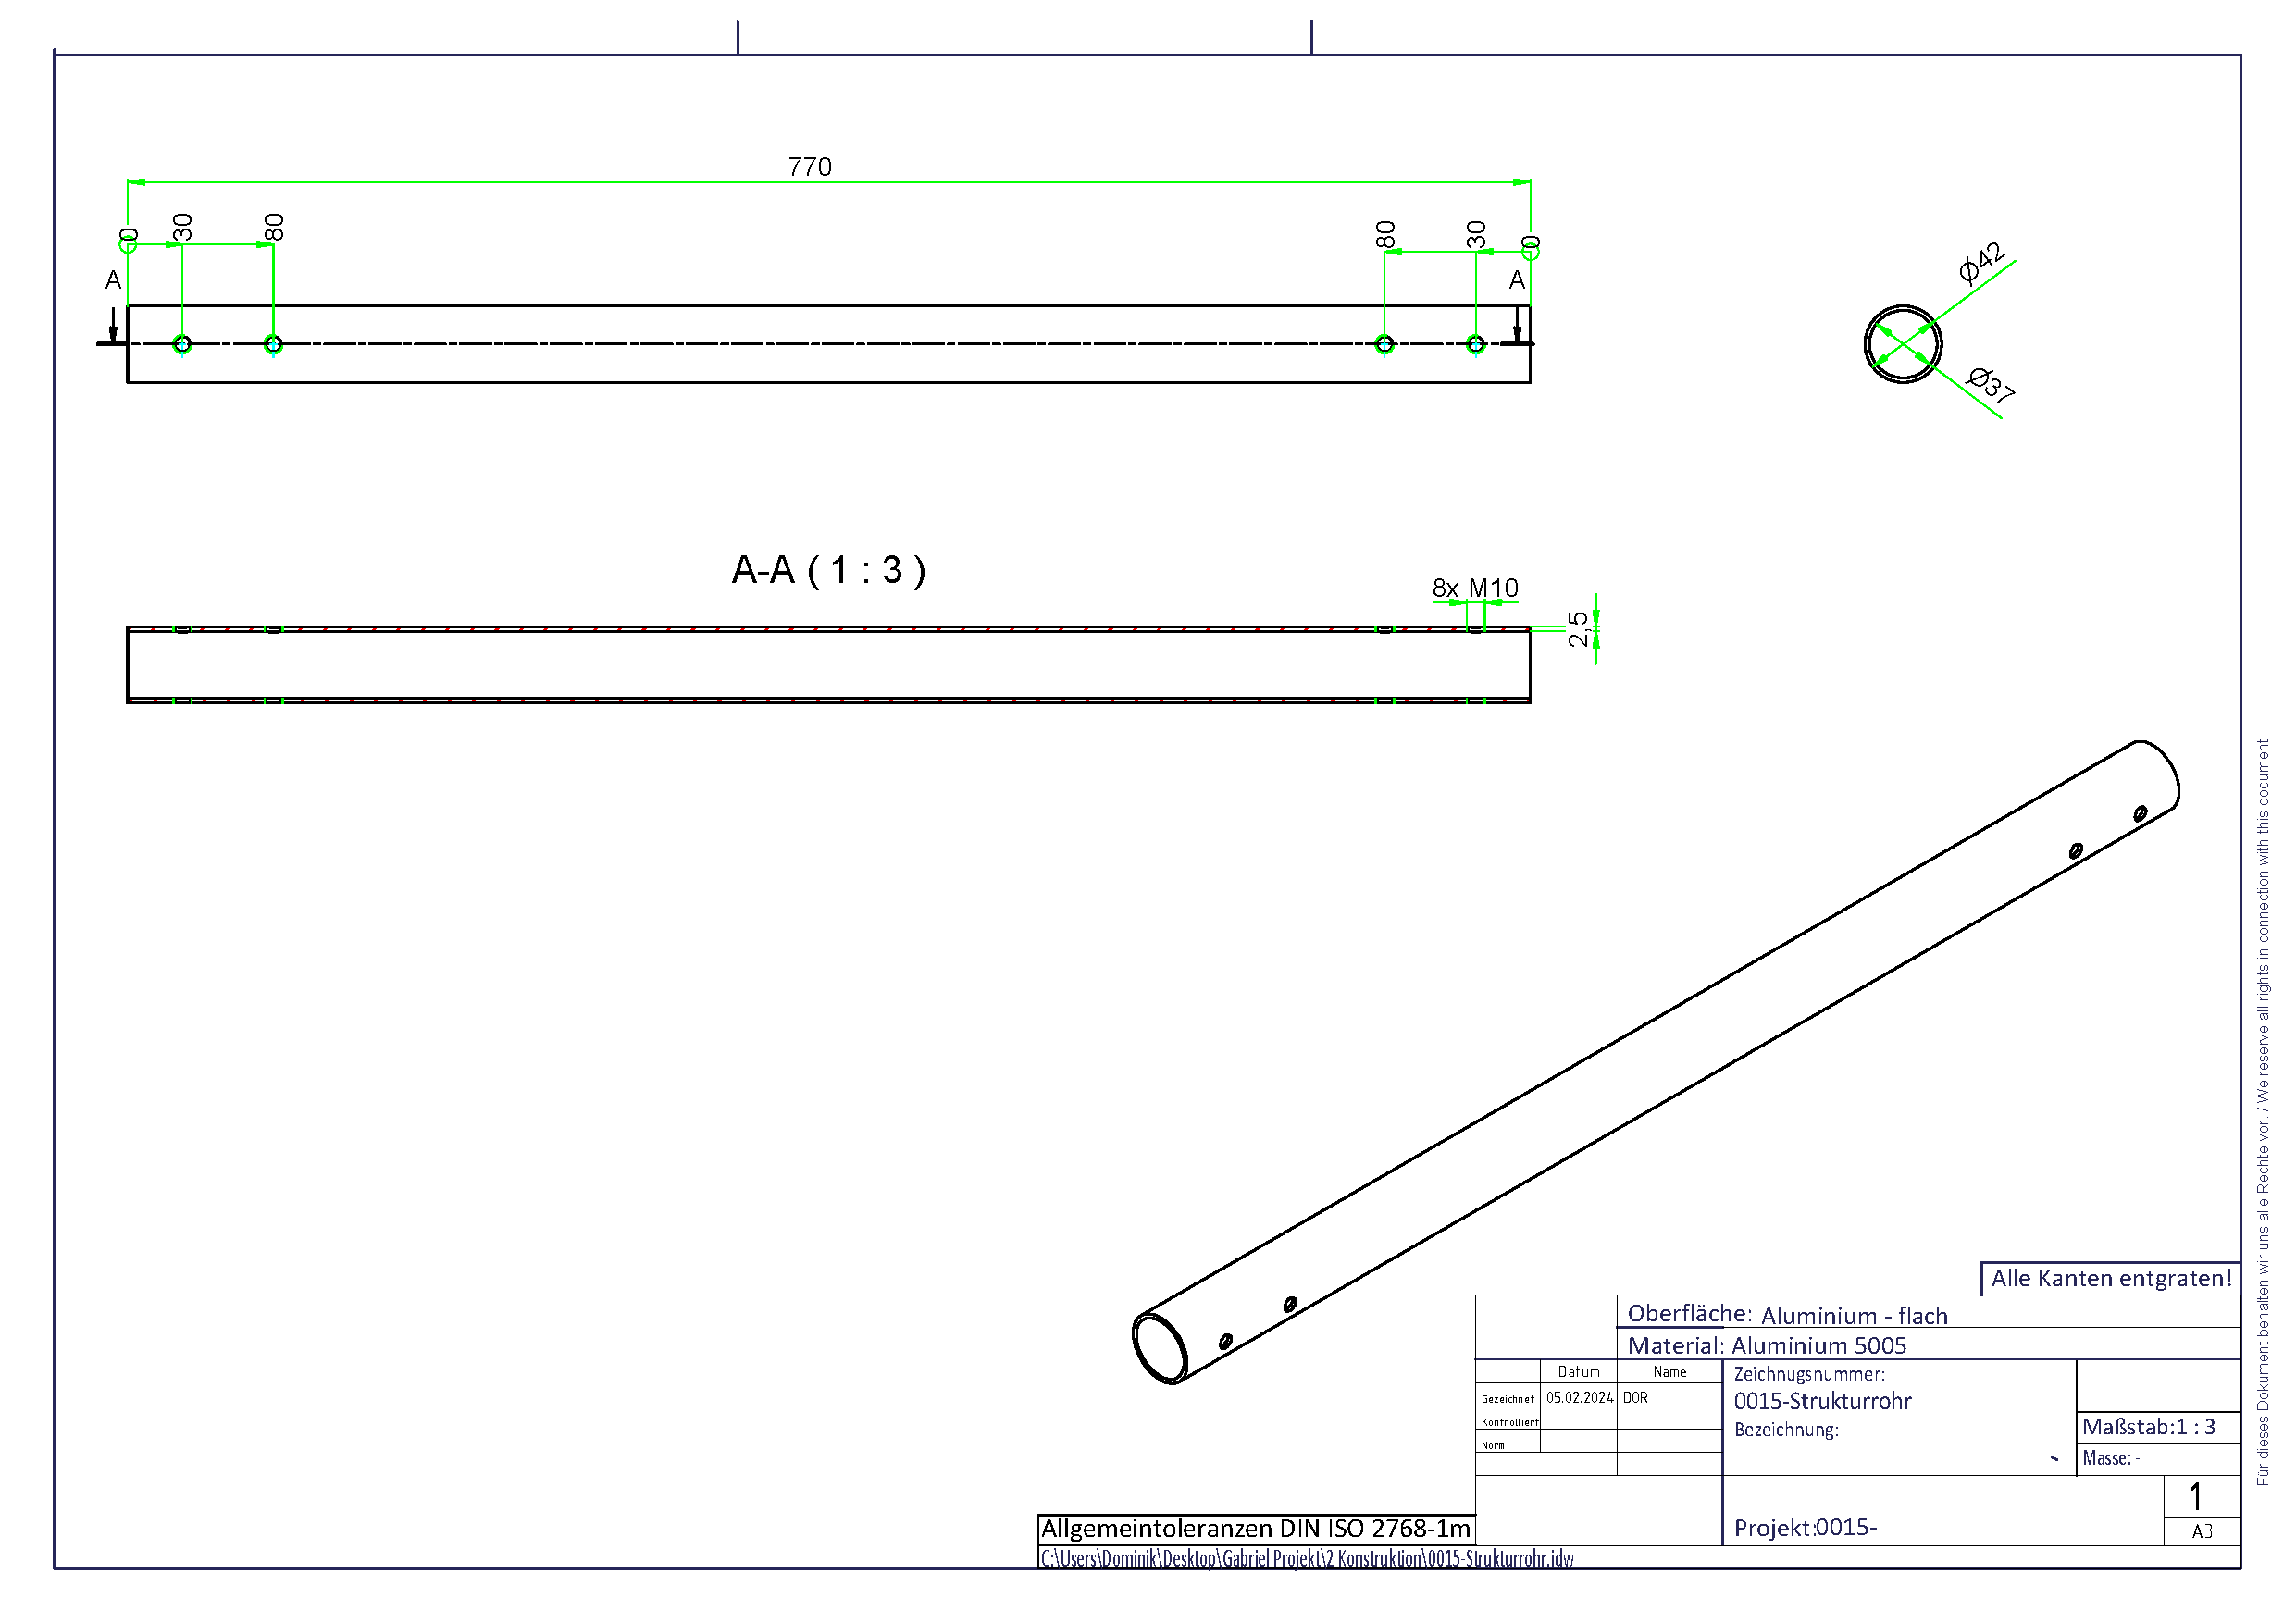
\includegraphics[angle=90,width=\textwidth]{../ref/0015-Strukturrohr.pdf}
	\caption{Zeichnung des Antennen Booms}
	\label{fig:Zeichnung-Antennenboom}
\end{figure}

\begin{figure}[h!]
	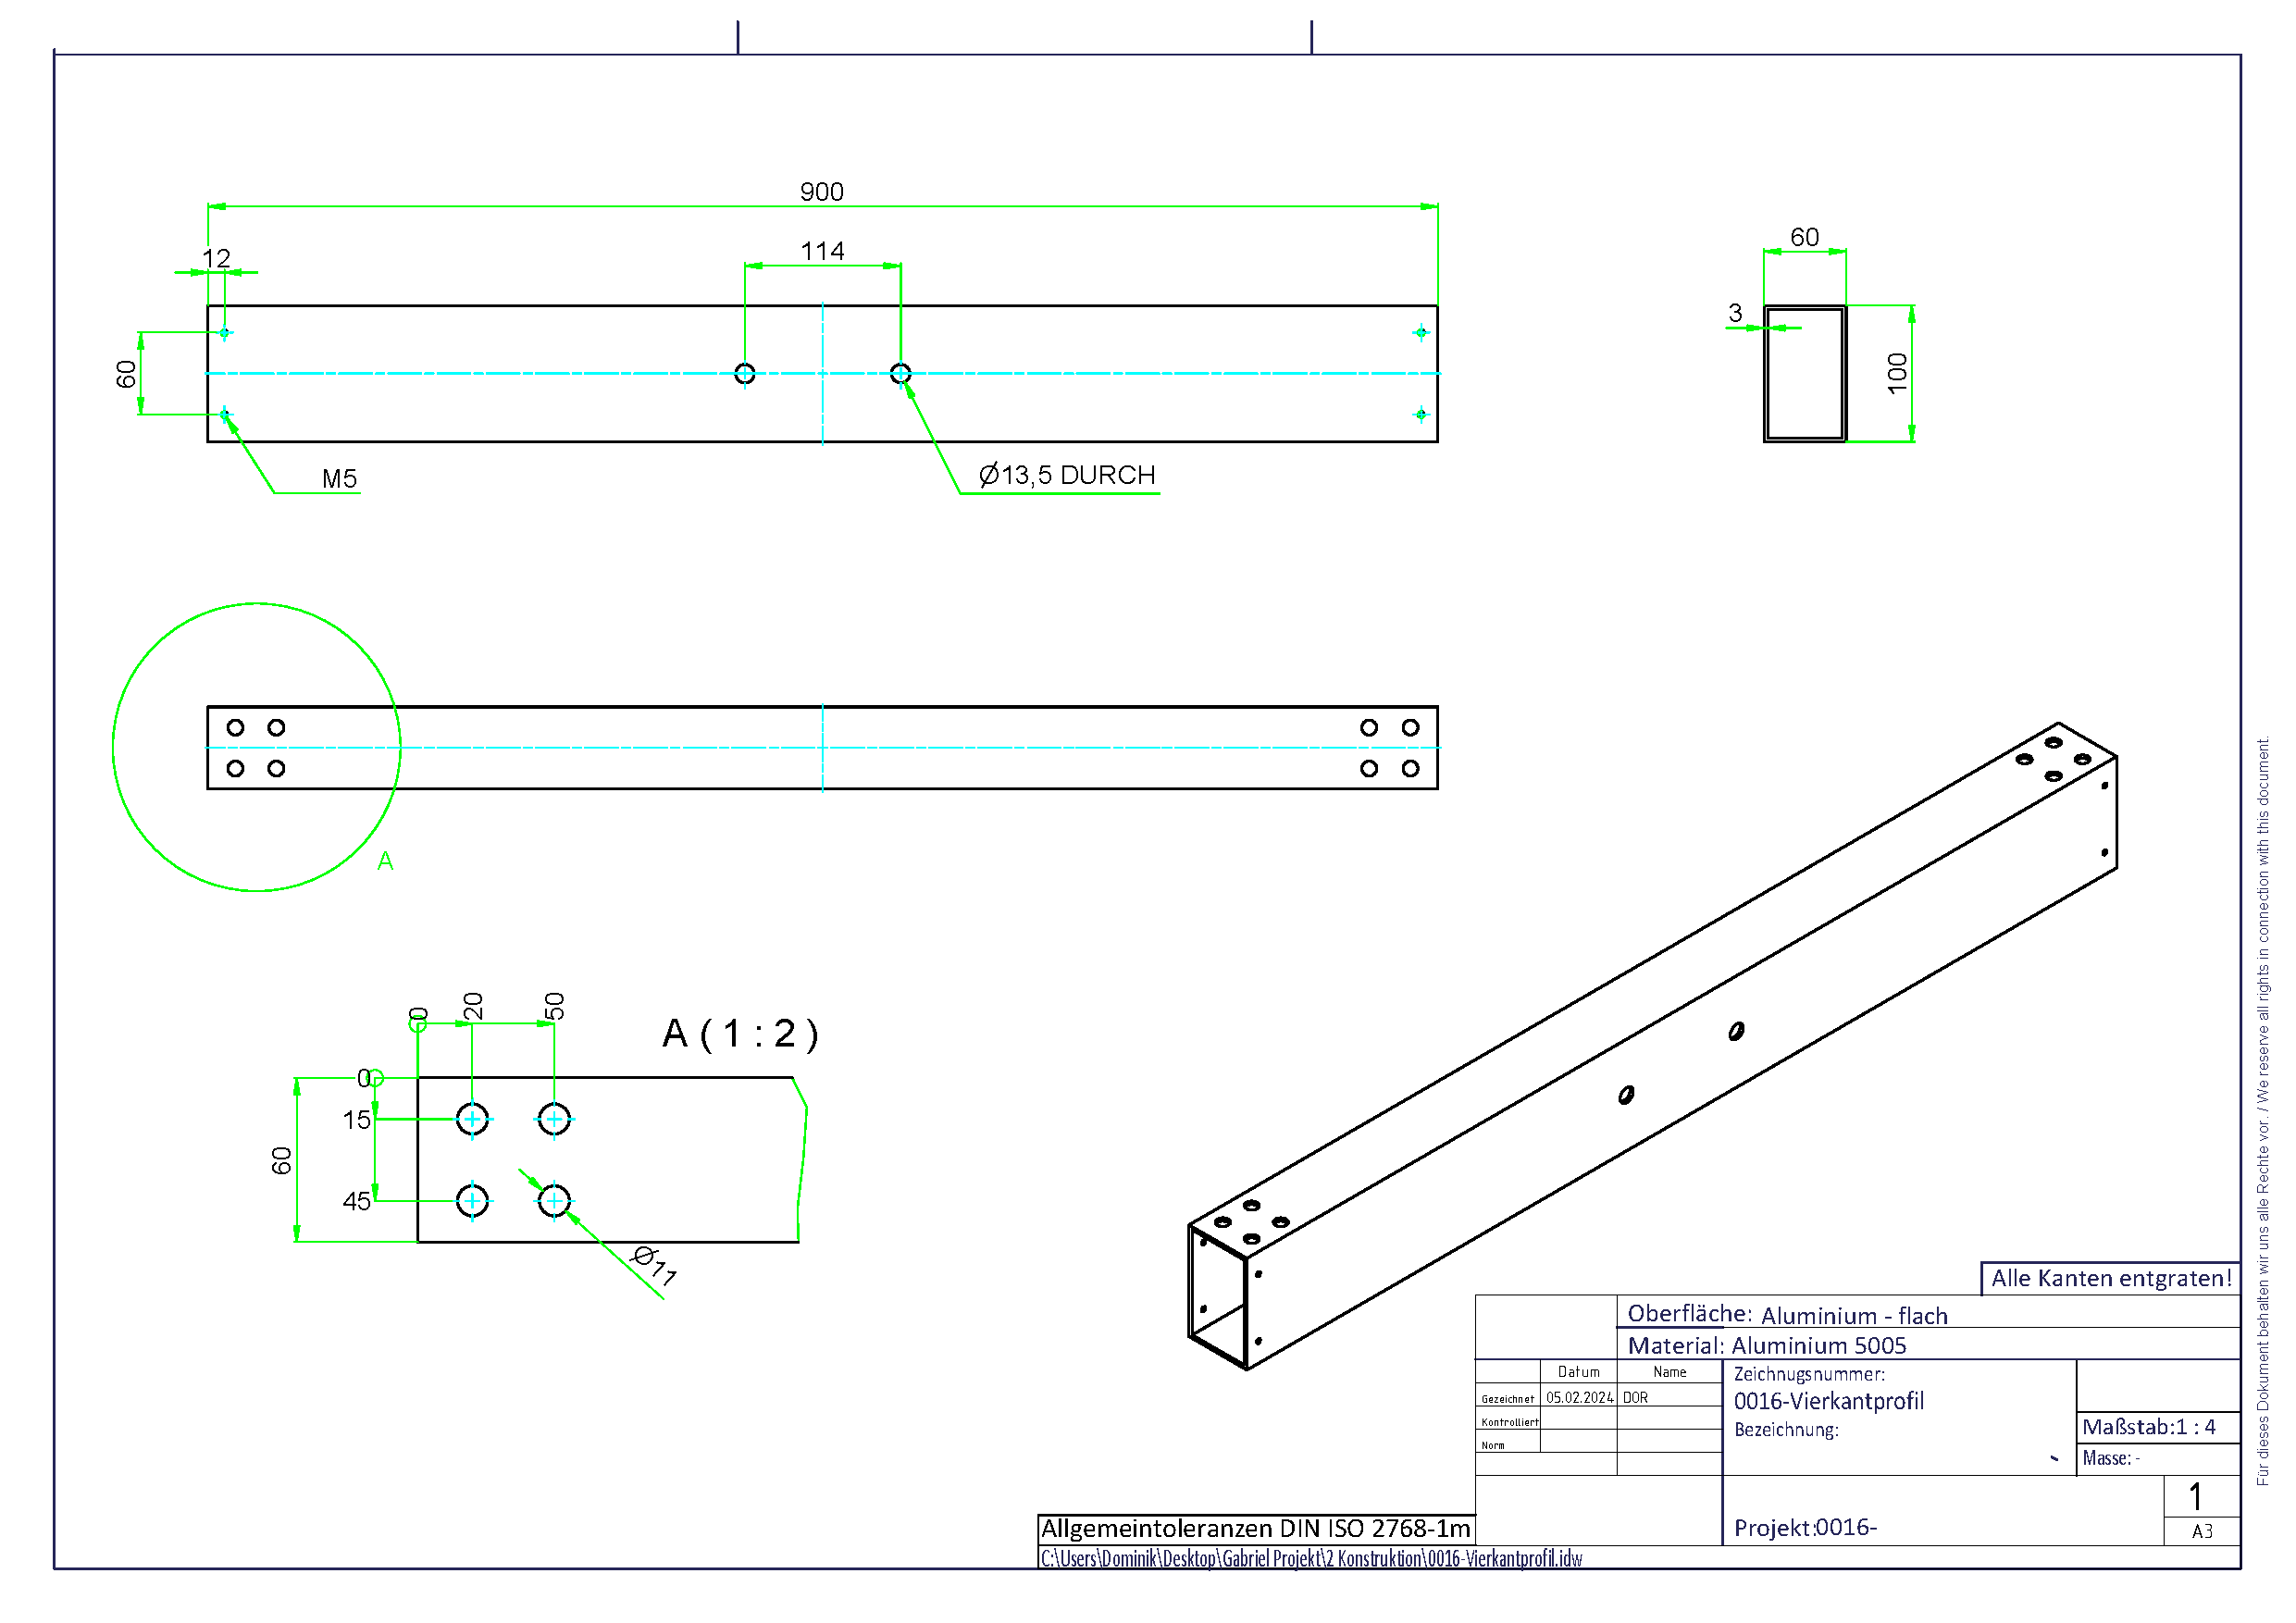
\includegraphics[angle=90,width=\textwidth]{../ref/0016-Vierkantprofil.pdf}
	\caption{Zeichnung des Vierkantrohres}
	\label{fig:Zeichnung-Vierkantrohr}
\end{figure}

\begin{figure}[h!]
	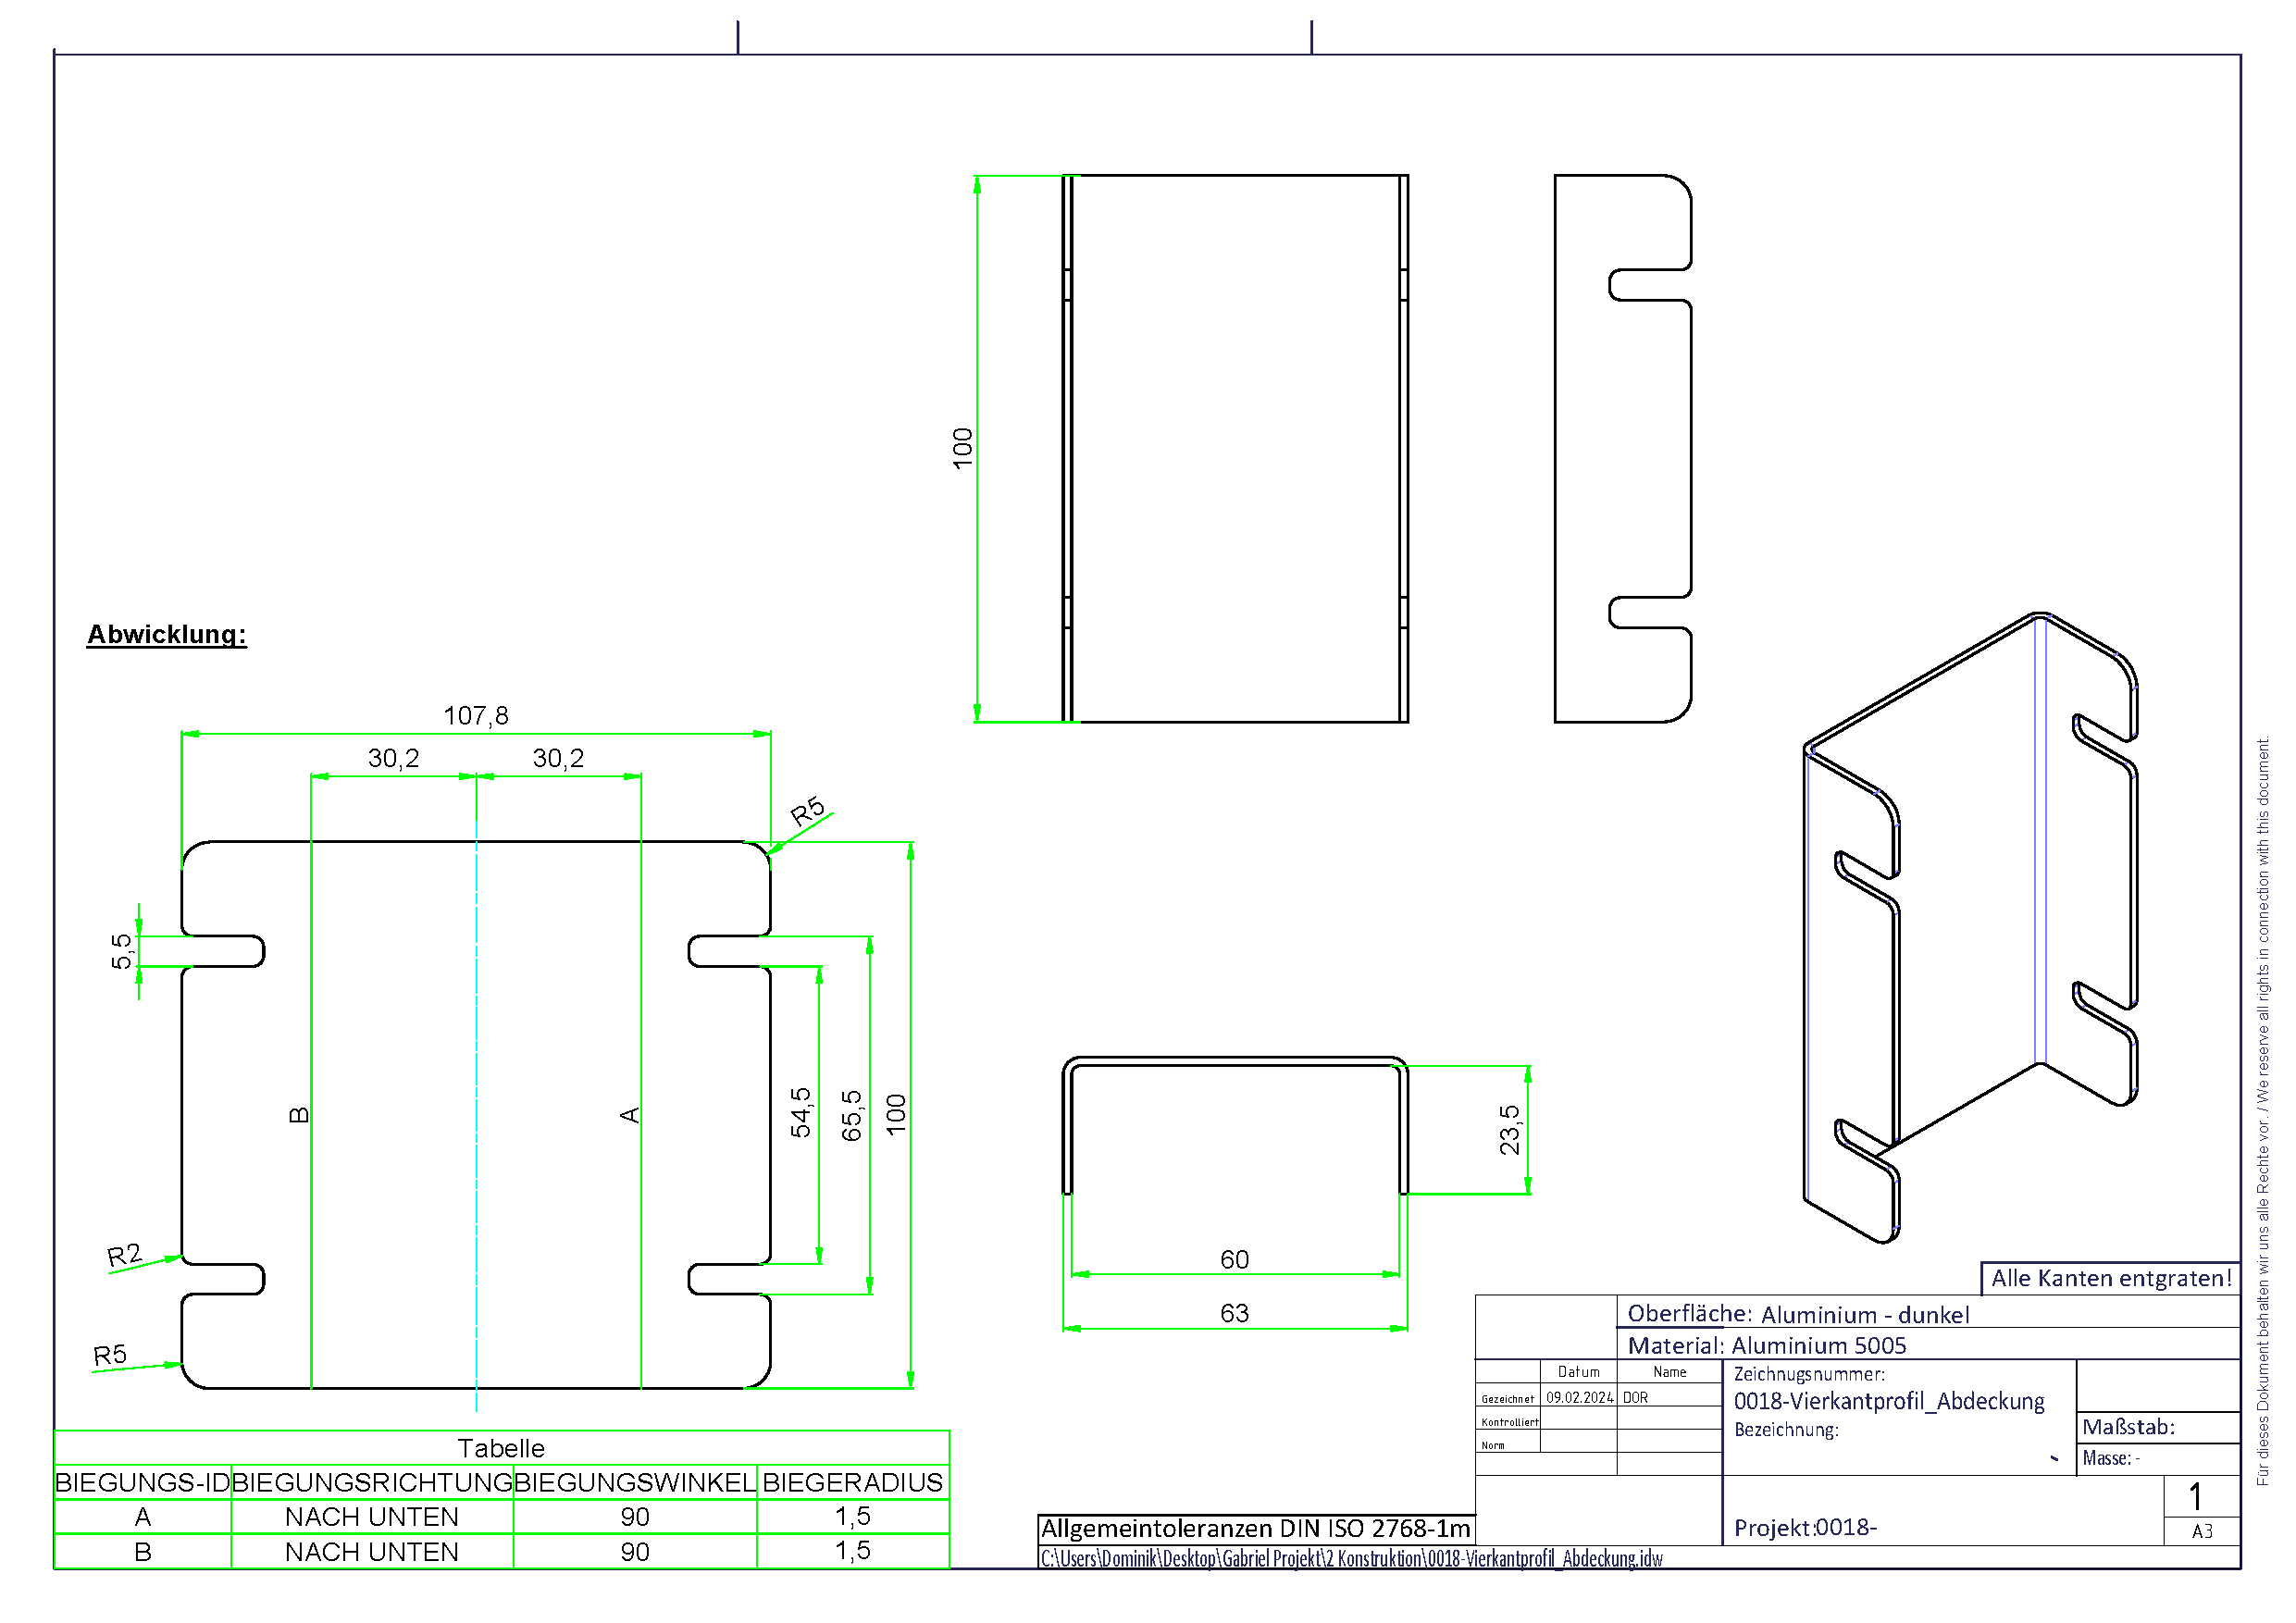
\includegraphics[angle=90,width=\textwidth]{../ref/0018-Vierkantprofil_Abdeckung.pdf}
	\caption{Zeichnung der Abdeckung des Vierkantrohres}
	\label{fig:Zeichnung-Vierkantrohr-Abdeckung}
\end{figure}

\begin{figure}[h!]
	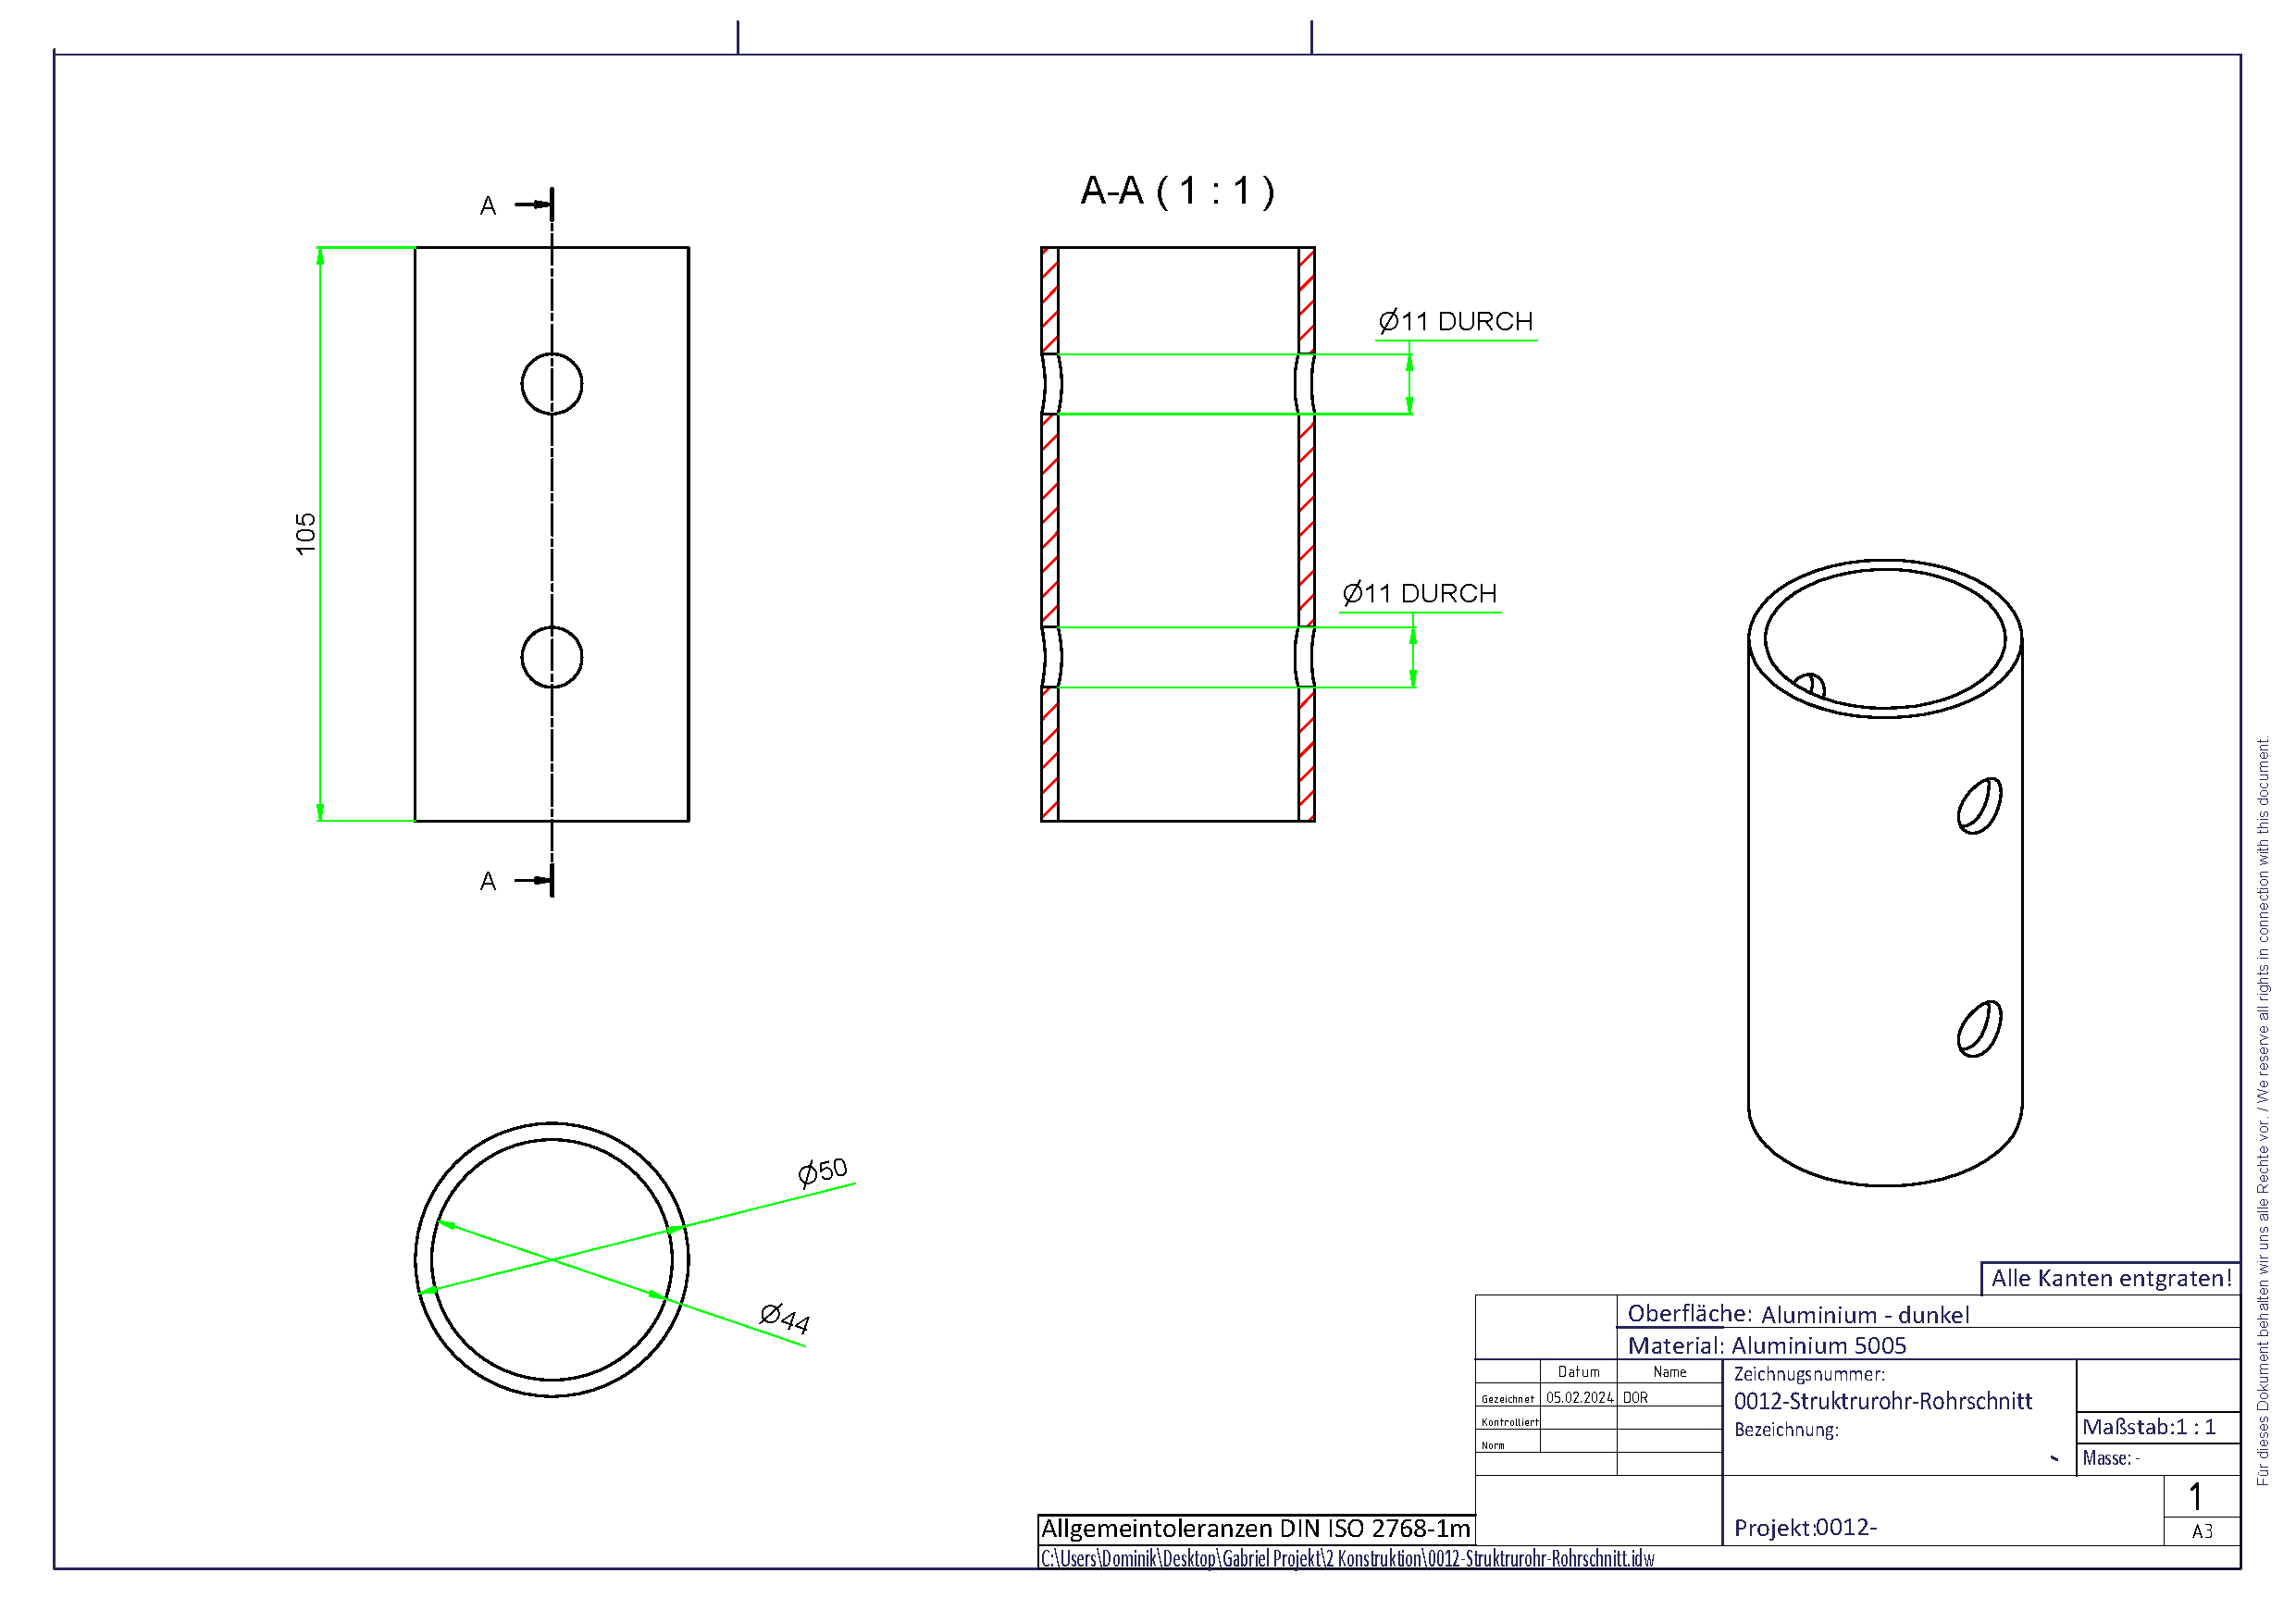
\includegraphics[angle=90,width=\textwidth]{../ref/0012-Struktrurohr-Rohrschnitt.pdf}
	\caption{Zeichnung des Rohrschnitts des Struktur-Rohrflansches}
	\label{fig:Zeichnung-Strukturrohrflansch-Rohrschnitt}
\end{figure}

\begin{figure}[h!]
	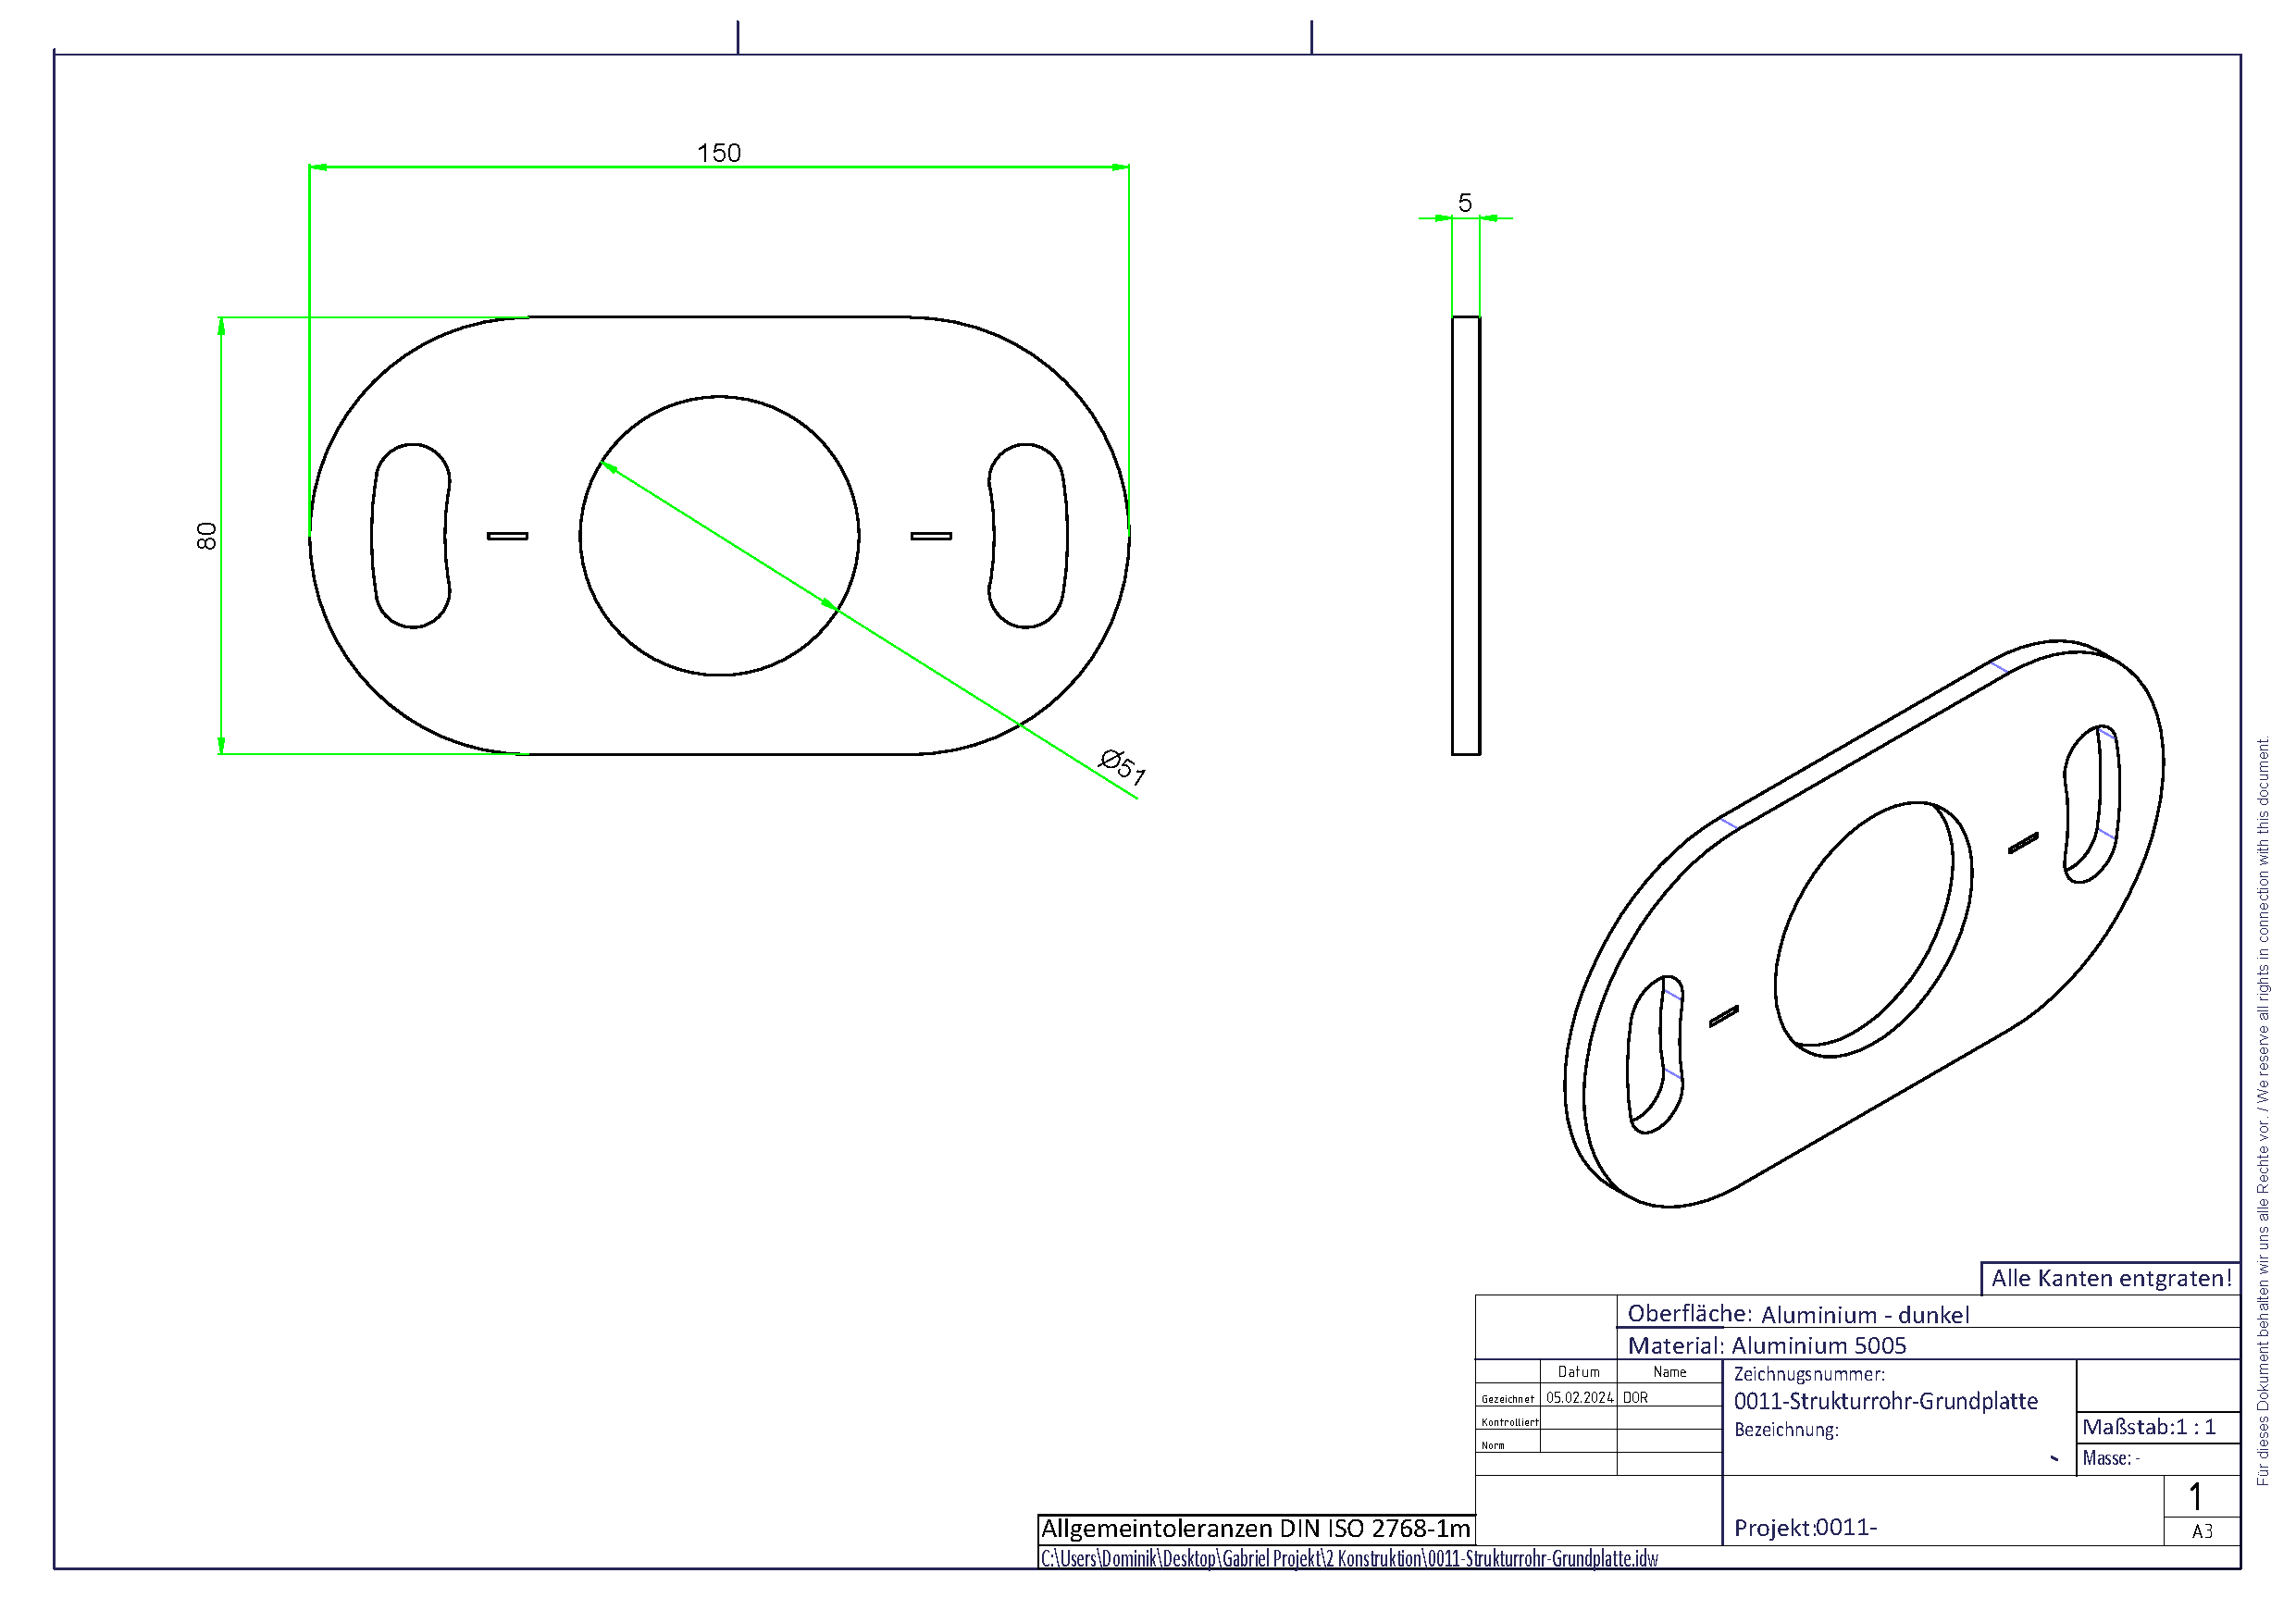
\includegraphics[angle=90,width=\textwidth]{../ref/0011-Strukturrohr-Grundplatte.pdf}
	\caption{Zeichnung der Grundplatte des Struktur-Rohrflansches}
	\label{fig:Zeichnung-Strukturrohrflansch-Grundplatte}
\end{figure}

\begin{figure}[h!]
	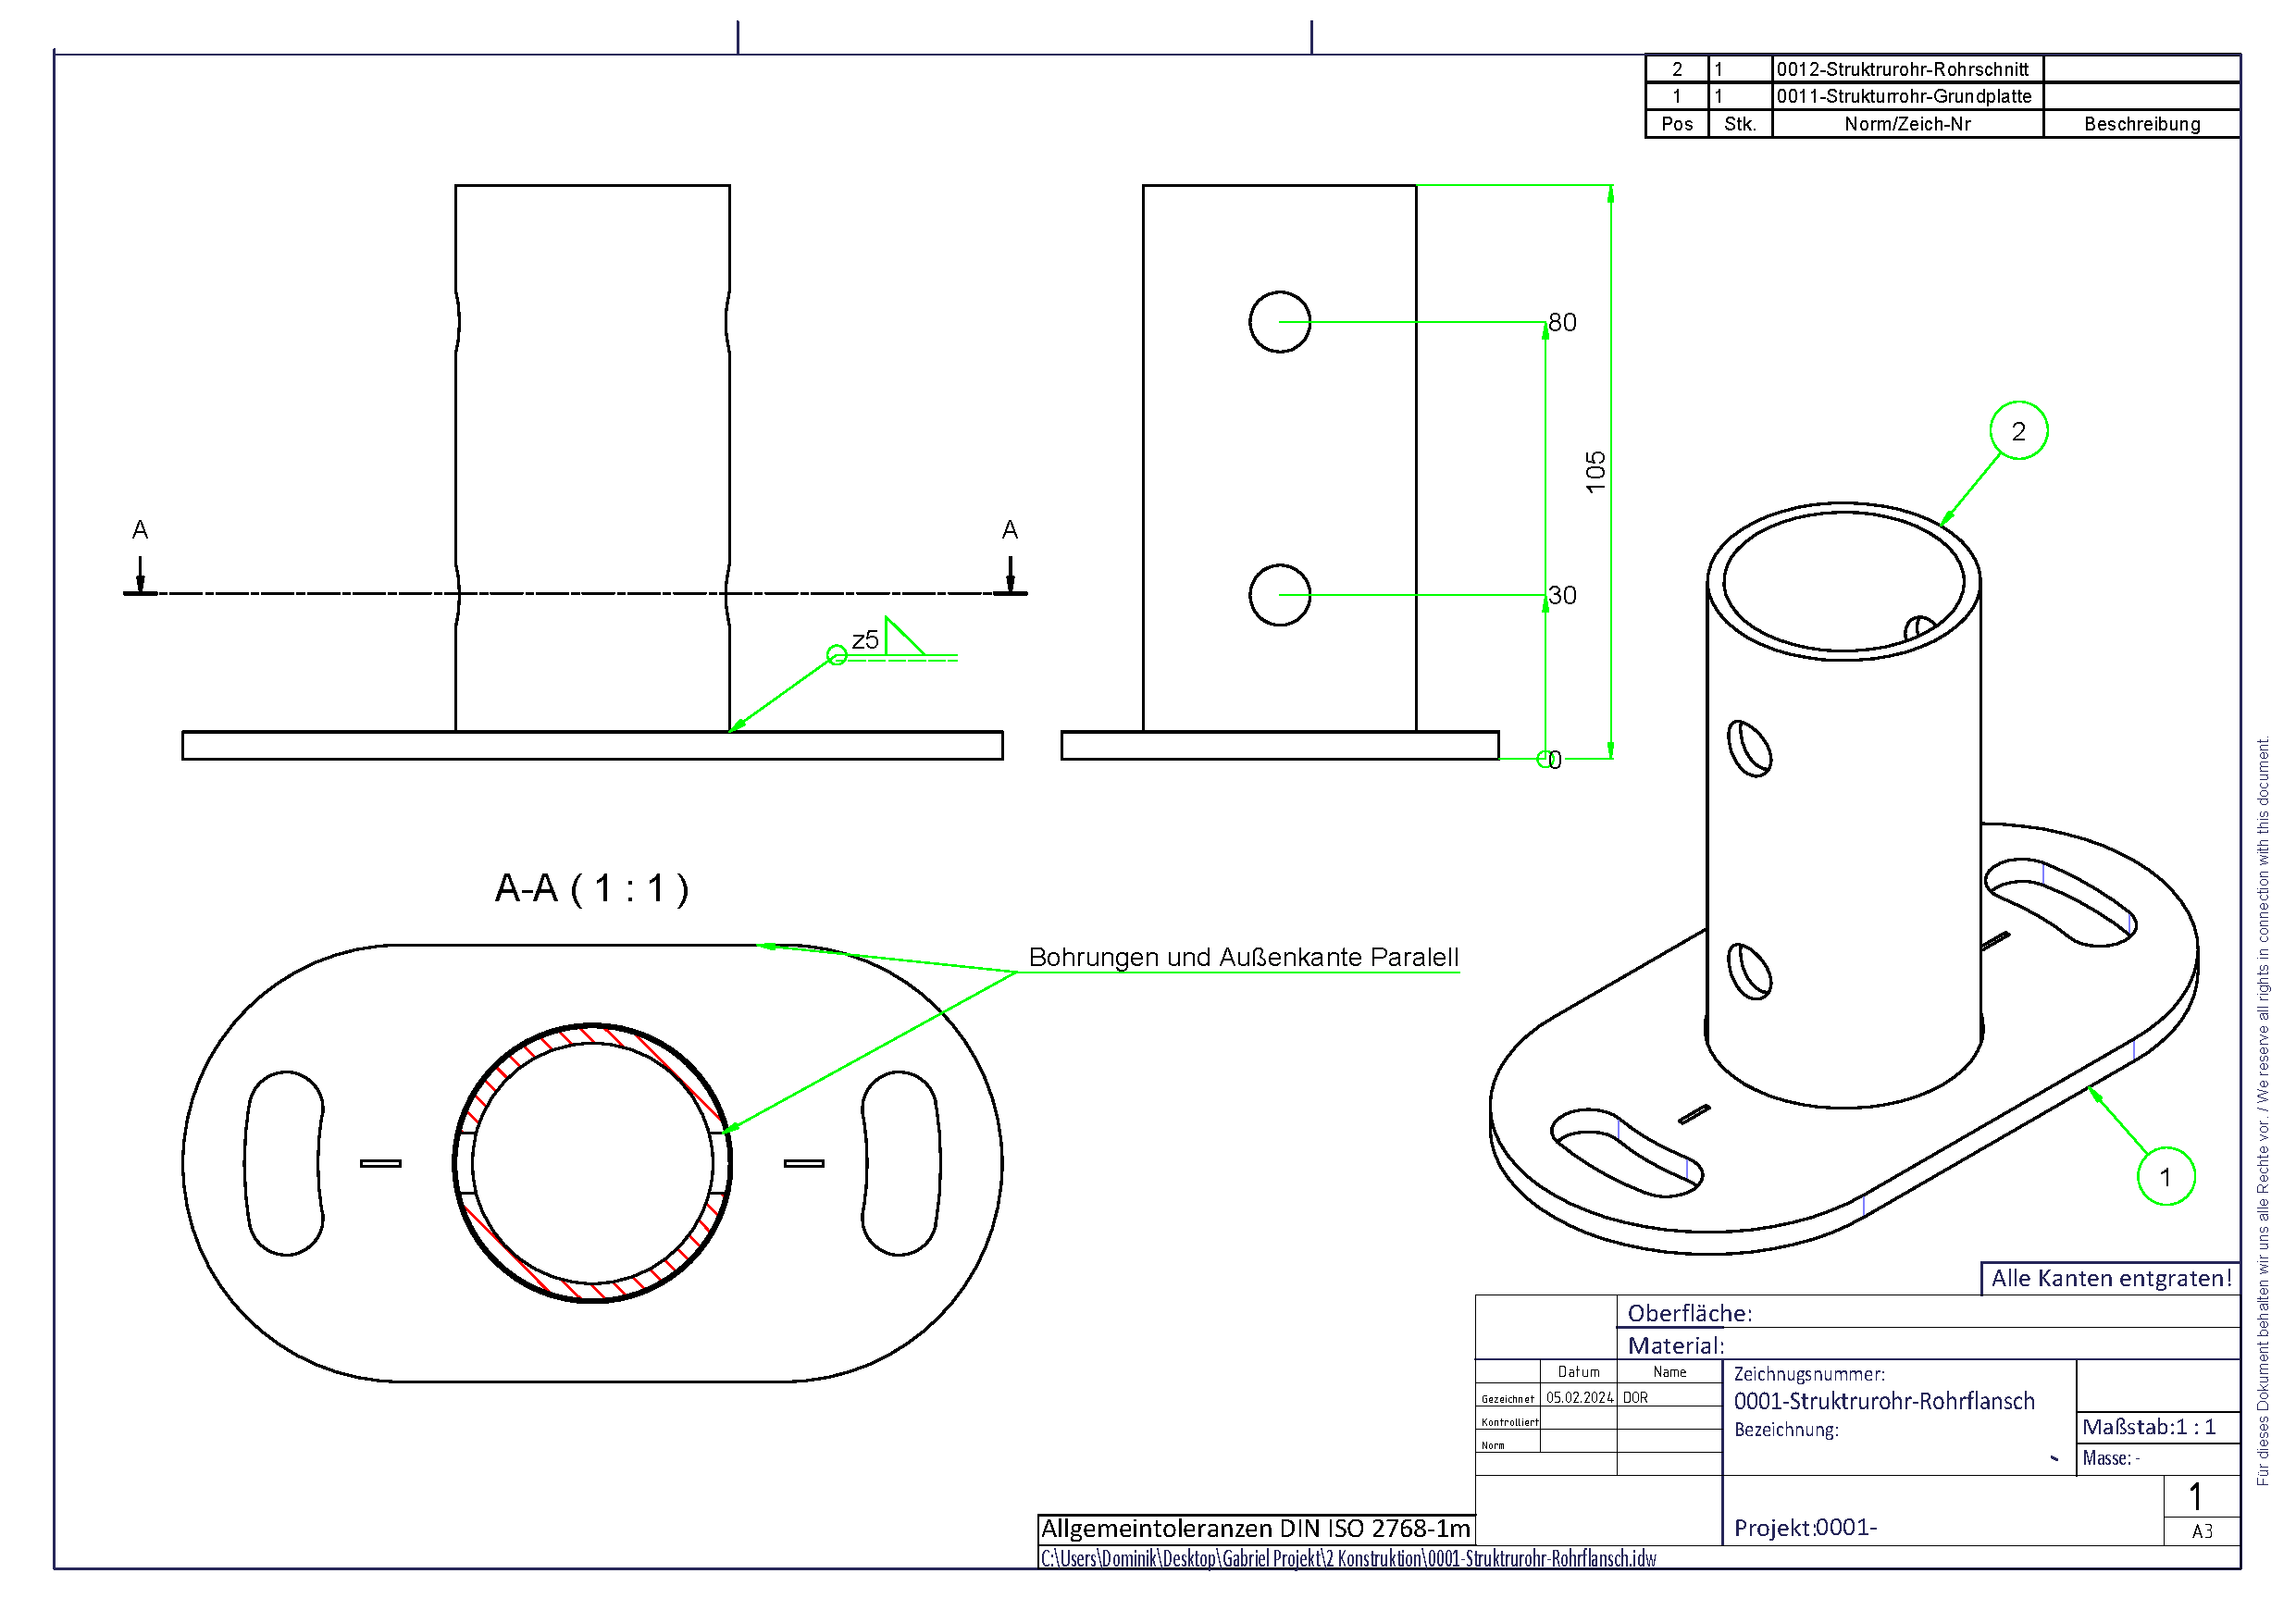
\includegraphics[angle=90,width=\textwidth]{../ref/0001-Struktrurohr-Rohrflansch.pdf}
	\caption{Zeichnung des Struktur-Rohrflansches}
	\label{fig:Zeichnung-Strukturrohrflansch}
\end{figure}

\begin{figure}[h!]
	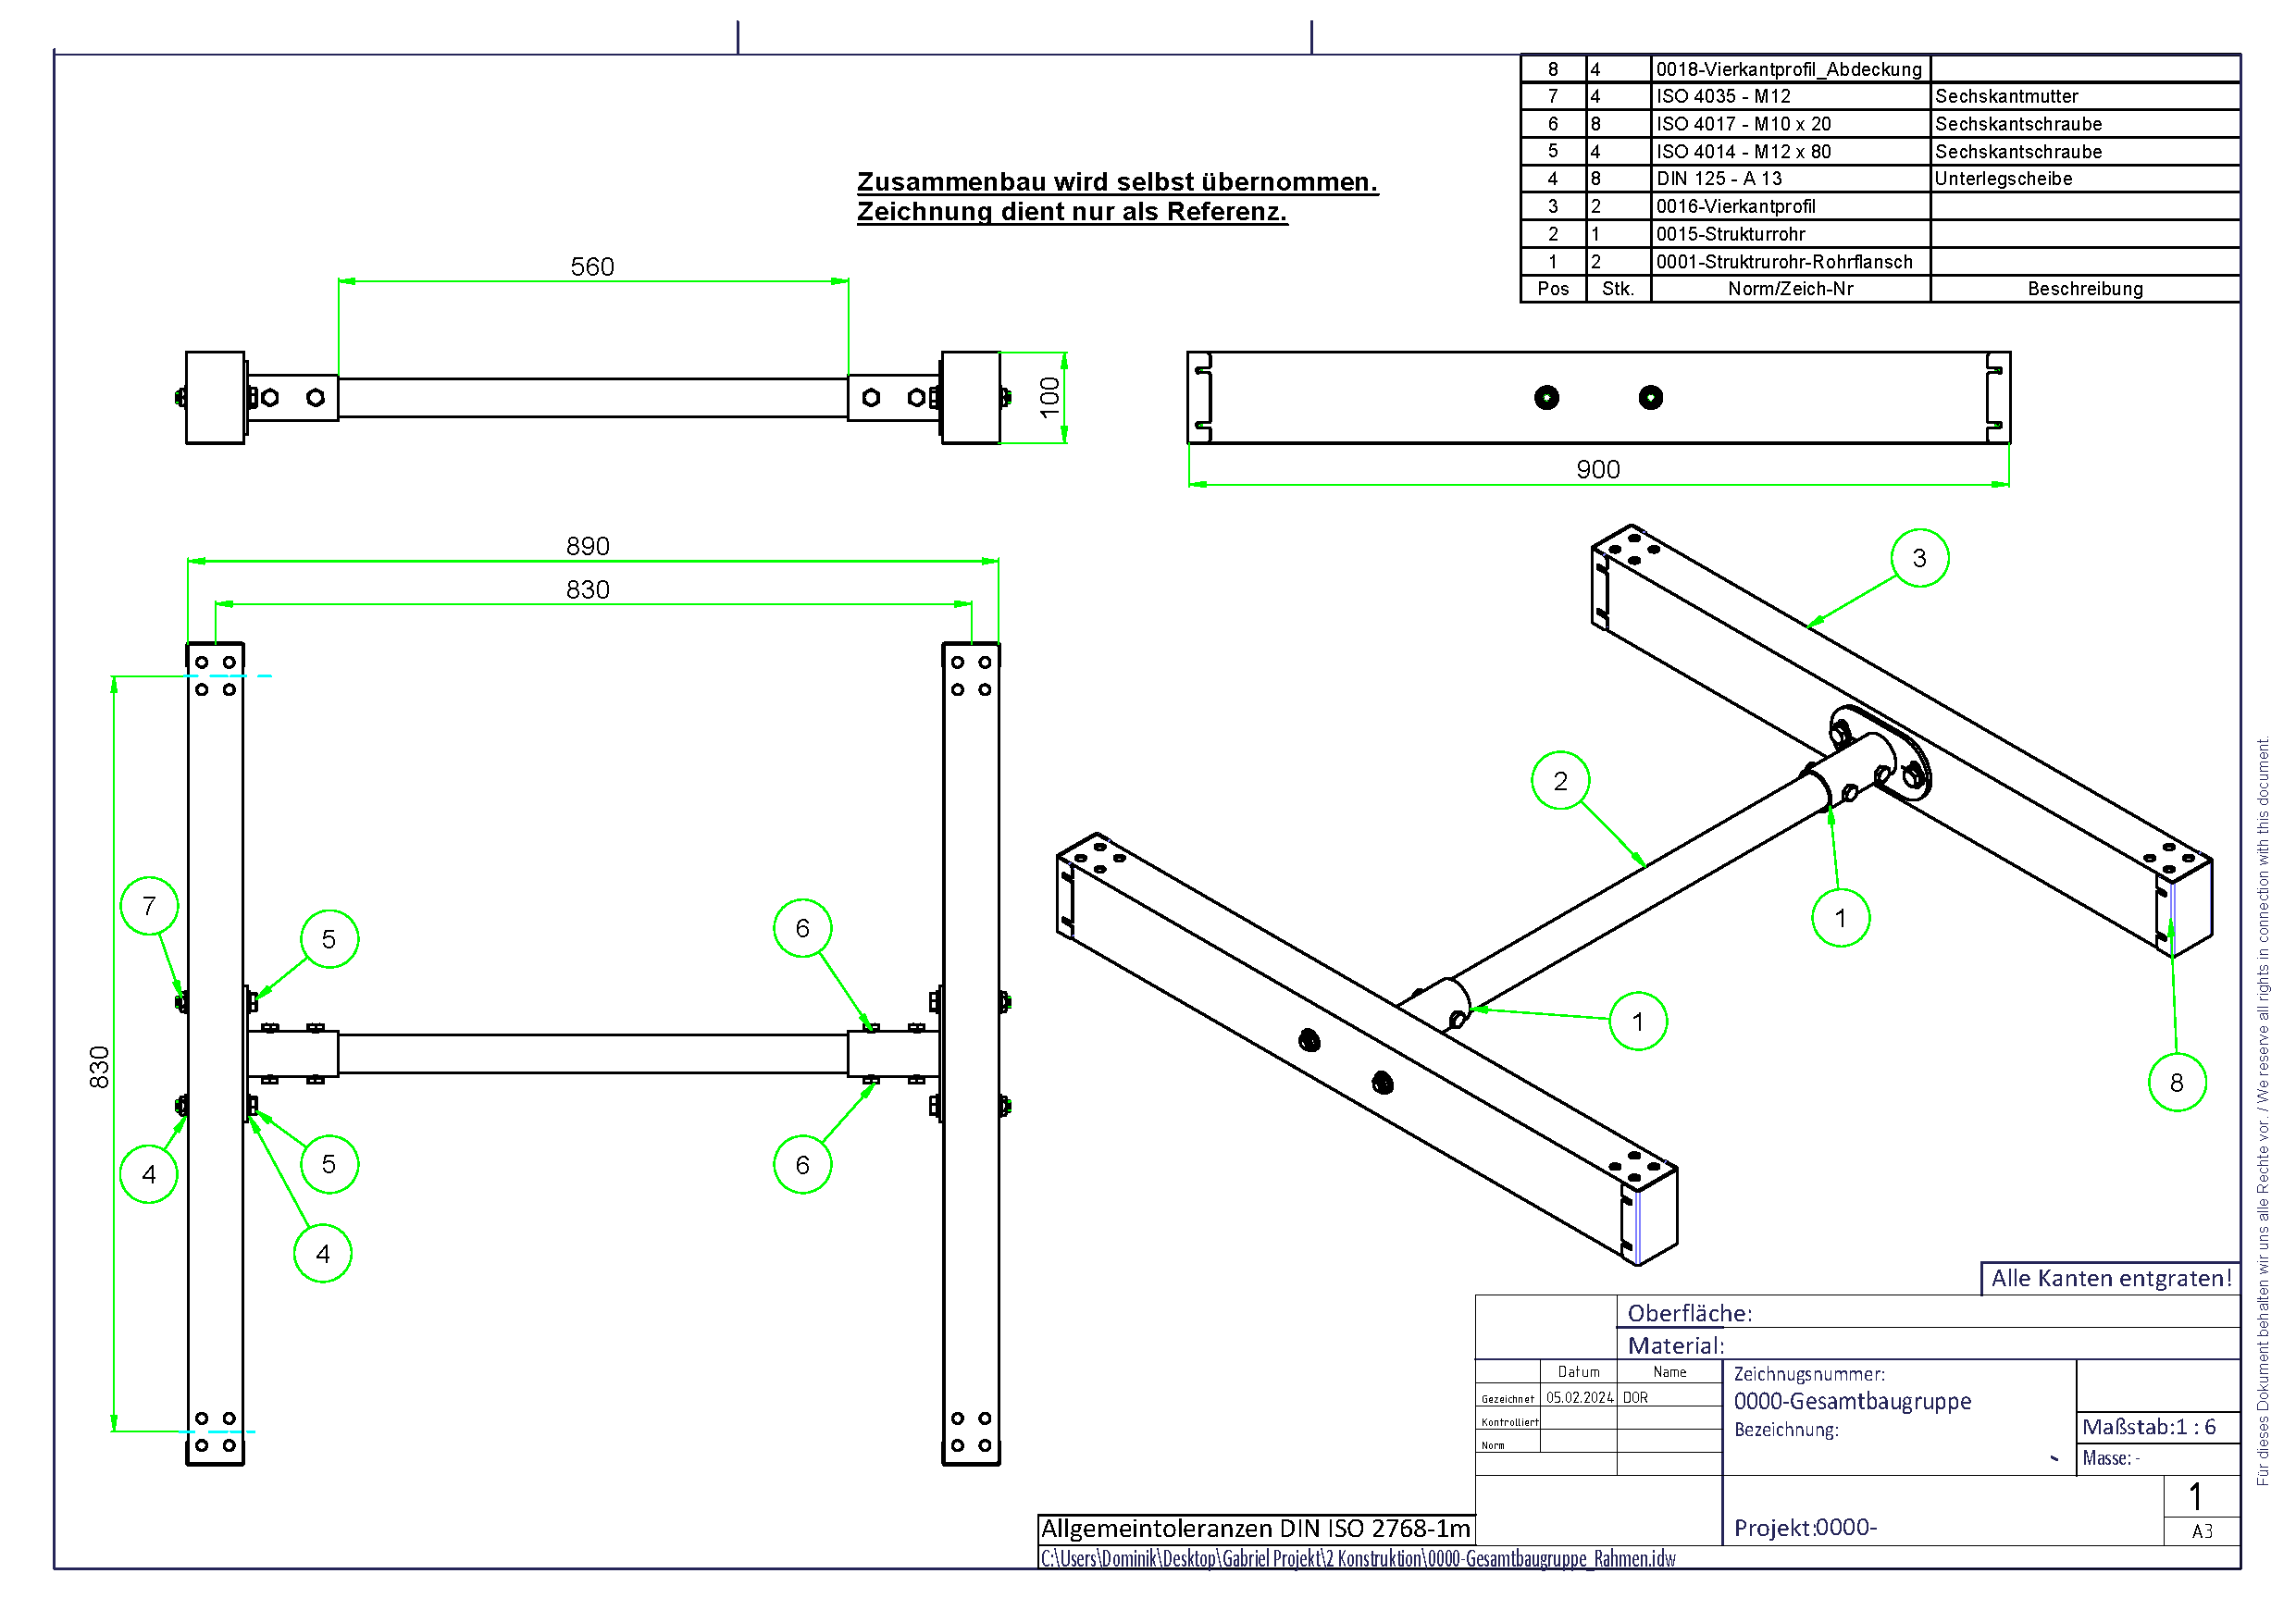
\includegraphics[angle=90,width=\textwidth]{../ref/0000-Gesamtbaugruppe_Rahmen.pdf}
	\caption{Zeichnung des Gerüsts}
	\label{fig:Zeichnung-Gerüst}
\end{figure}

\begin{figure}[h!]
	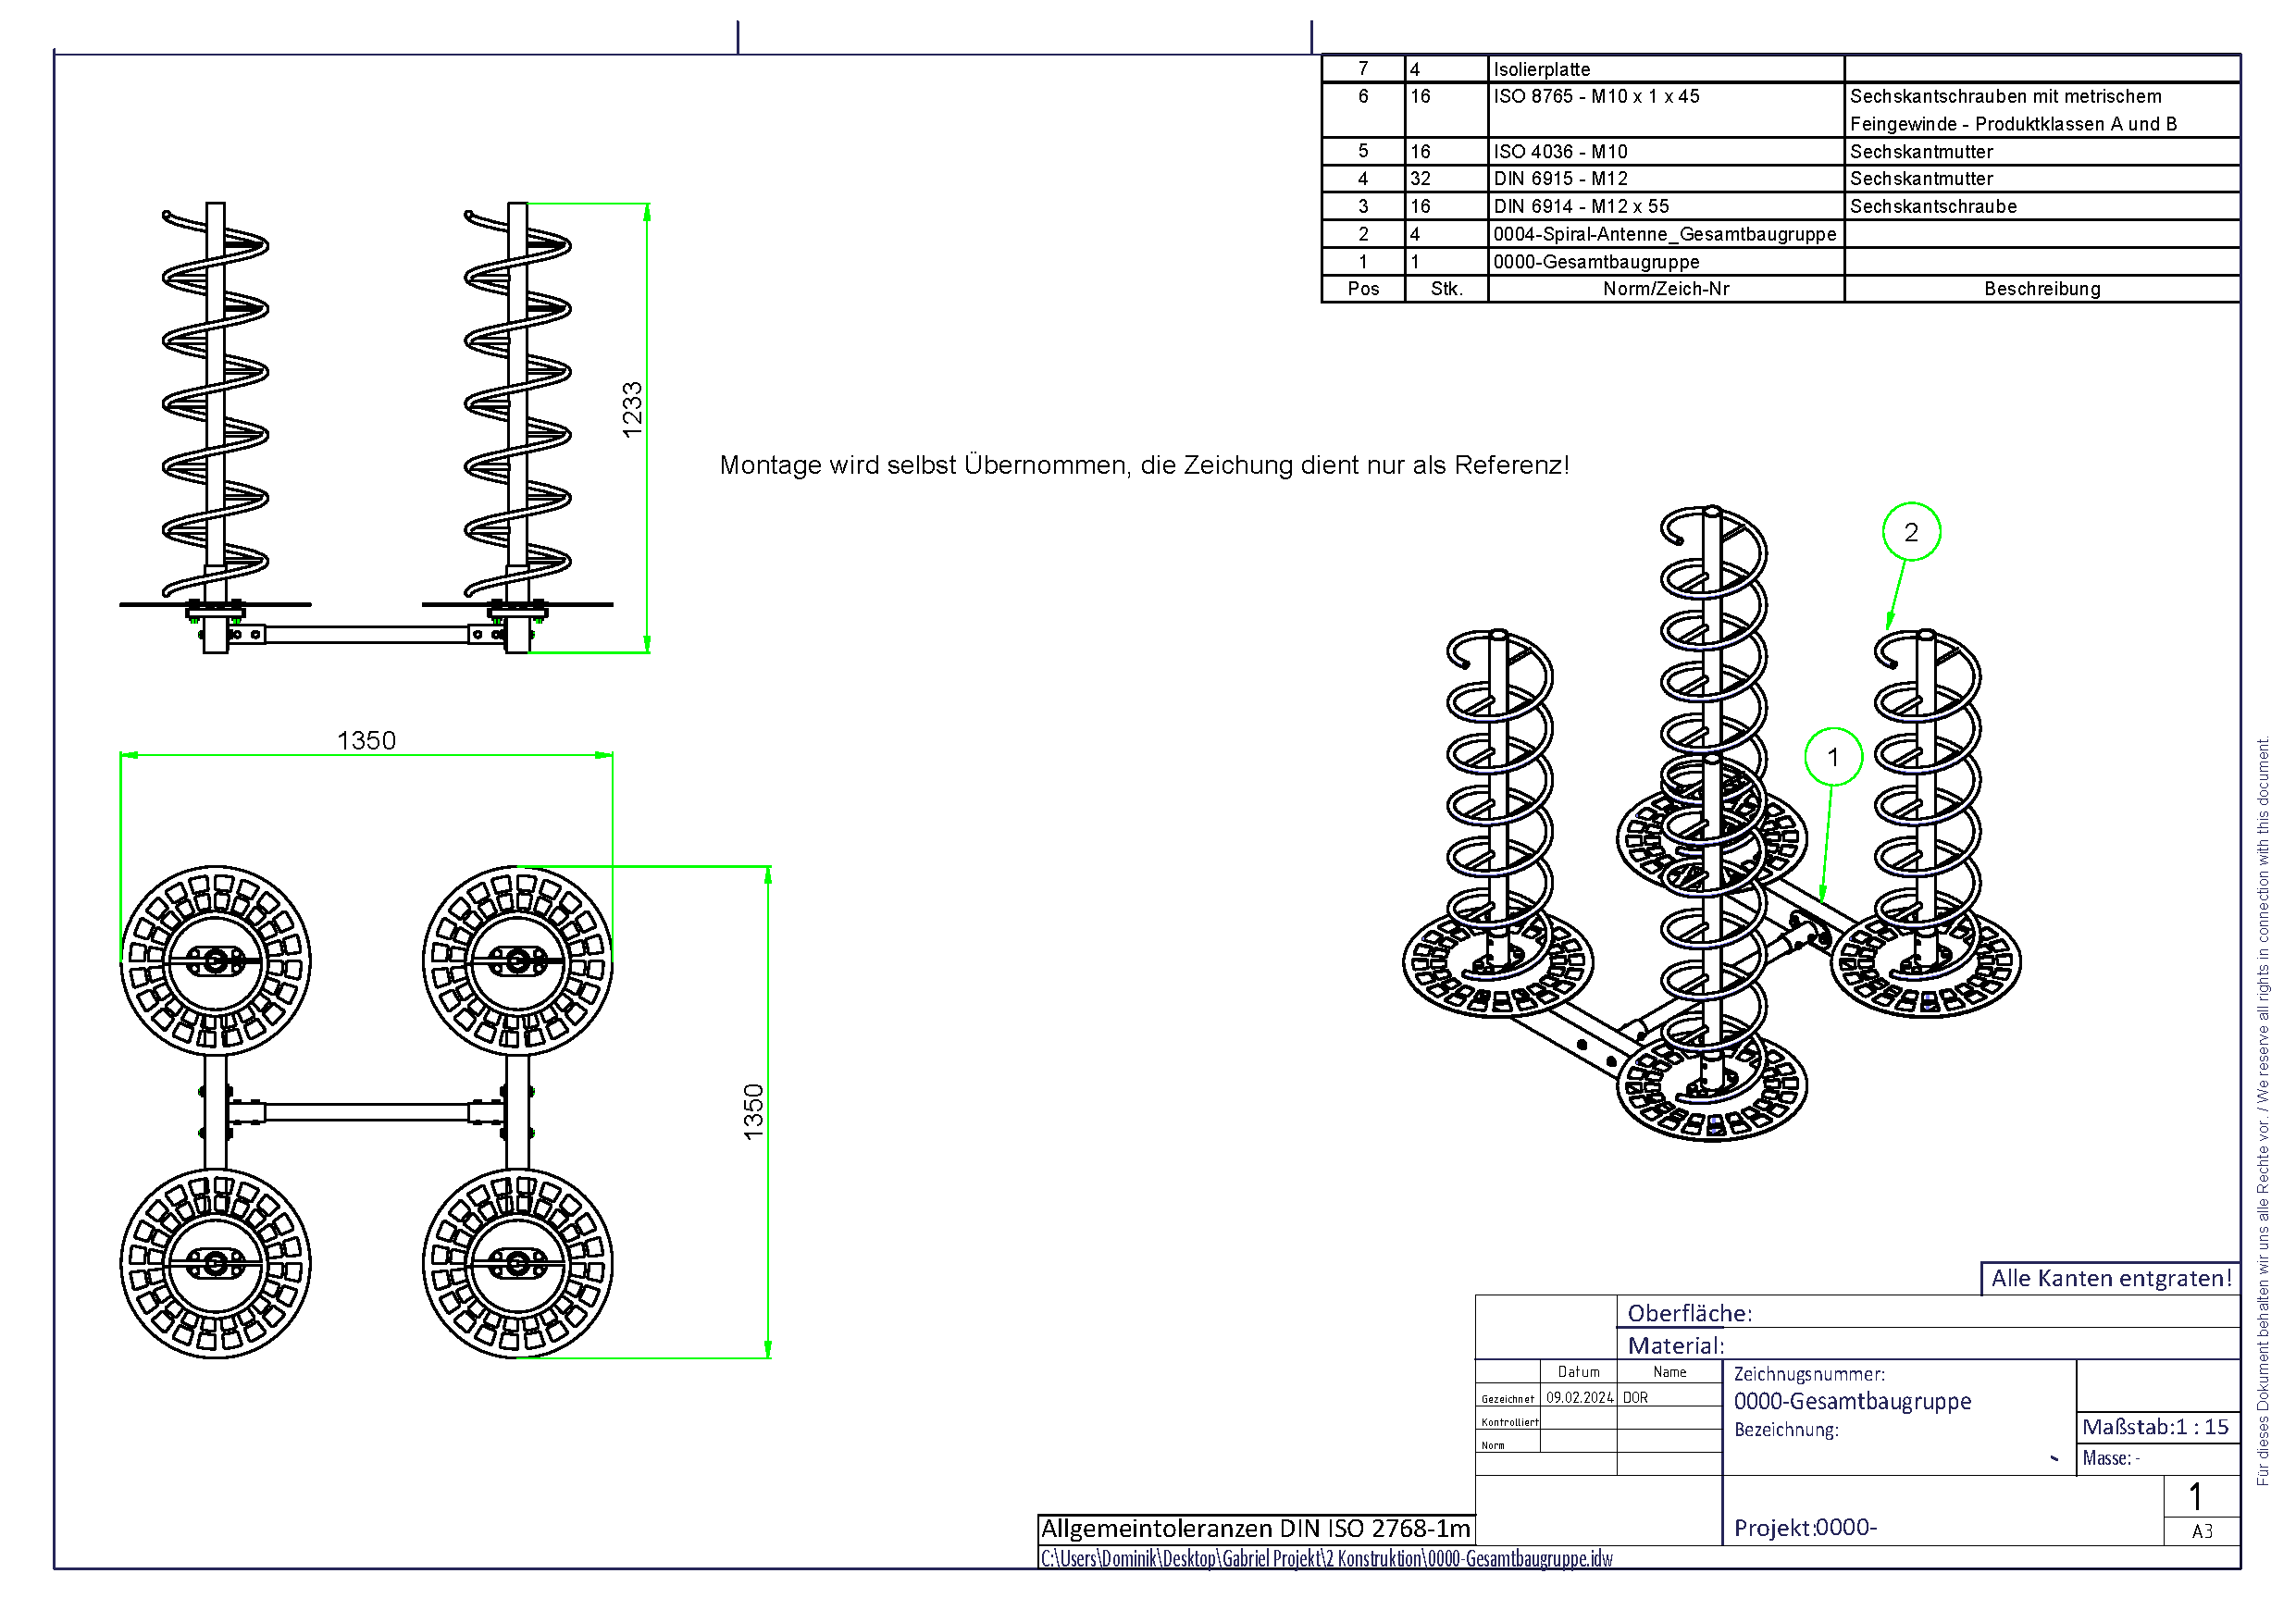
\includegraphics[angle=90,width=\textwidth]{../ref/0000-Gesamtbaugruppe.pdf}
	\caption{Zeichnung des Antennenarrays}
	\label{fig:Zeichnung-Antennenarray}
\end{figure}

